% SDIA2026_SAN-1_GROUP_13 -- IEEE conference article (Overleaf: compile with pdfLaTeX).
% Prose is hand-written. Every result value is a \val... macro from numbers.tex, which
% scripts/make_latex.py generates from paper/numbers*.json; tables/ are generated too.
% scripts/audit_latex.py refuses any literal result number in this file.
\documentclass[conference,a4paper]{IEEEtran}
\IEEEoverridecommandlockouts

\usepackage{cite}
\usepackage{amsmath}
\usepackage{amssymb}
\usepackage{graphicx}
\usepackage{booktabs}
\usepackage{url}
\usepackage{xspace}
\xspaceaddexceptions{\%}

% Generated by scripts/make_latex.py from paper/numbers*.json. Do not edit.
% Every macro is one value produced from results/ or the frozen contract.

\newcommand{\valAblationLoraLastTwoOneAucIn}{0.752 $\pm$ 0.106\xspace}% ablation.lora_last2.1.auc_in
\newcommand{\valAblationLoraLastTwoOneAucOut}{0.530 $\pm$ 0.042\xspace}% ablation.lora_last2.1.auc_out
\newcommand{\valAblationLoraLastTwoOneVsLoRAIn}{+0.012\xspace}% ablation.lora_last2.1.vs_LoRA.in
\newcommand{\valAblationLoraLastTwoOneVsLoRAOut}{$-$0.071\xspace}% ablation.lora_last2.1.vs_LoRA.out
\newcommand{\valAblationLoraLastTwoOneVsPFTIn}{$-$0.018\xspace}% ablation.lora_last2.1.vs_PFT.in
\newcommand{\valAblationLoraLastTwoOneVsPFTOut}{$-$0.020\xspace}% ablation.lora_last2.1.vs_PFT.out
\newcommand{\valAblationLoraLastTwoTenAucIn}{0.846 $\pm$ 0.078\xspace}% ablation.lora_last2.10.auc_in
\newcommand{\valAblationLoraLastTwoTenAucOut}{0.521 $\pm$ 0.058\xspace}% ablation.lora_last2.10.auc_out
\newcommand{\valAblationLoraLastTwoTenVsLoRAIn}{$-$0.053\xspace}% ablation.lora_last2.10.vs_LoRA.in
\newcommand{\valAblationLoraLastTwoTenVsLoRAOut}{$-$0.188\xspace}% ablation.lora_last2.10.vs_LoRA.out
\newcommand{\valAblationLoraLastTwoTenVsPFTIn}{+0.021\xspace}% ablation.lora_last2.10.vs_PFT.in
\newcommand{\valAblationLoraLastTwoTenVsPFTOut}{$-$0.061\xspace}% ablation.lora_last2.10.vs_PFT.out
\newcommand{\valAblationLoraLastTwoHundredAucIn}{0.942 $\pm$ 0.008\xspace}% ablation.lora_last2.100.auc_in
\newcommand{\valAblationLoraLastTwoHundredAucOut}{0.763 $\pm$ 0.016\xspace}% ablation.lora_last2.100.auc_out
\newcommand{\valAblationLoraLastTwoHundredVsLoRAIn}{$-$0.016\xspace}% ablation.lora_last2.100.vs_LoRA.in
\newcommand{\valAblationLoraLastTwoHundredVsLoRAOut}{$-$0.042\xspace}% ablation.lora_last2.100.vs_LoRA.out
\newcommand{\valAblationLoraLastTwoHundredVsPFTIn}{$-$0.002\xspace}% ablation.lora_last2.100.vs_PFT.in
\newcommand{\valAblationLoraLastTwoHundredVsPFTOut}{$-$0.000\xspace}% ablation.lora_last2.100.vs_PFT.out
\newcommand{\valAblationLoraNoAugmentationTenAucIn}{0.845 $\pm$ 0.069\xspace}% ablation.lora_no_augmentation.10.auc_in
\newcommand{\valAblationLoraNoAugmentationTenAucOut}{0.629 $\pm$ 0.121\xspace}% ablation.lora_no_augmentation.10.auc_out
\newcommand{\valAblationLoraNoAugmentationTenVsLoRAIn}{$-$0.054\xspace}% ablation.lora_no_augmentation.10.vs_LoRA.in
\newcommand{\valAblationLoraNoAugmentationTenVsLoRAOut}{$-$0.080\xspace}% ablation.lora_no_augmentation.10.vs_LoRA.out
\newcommand{\valAblationLoraRankSixteenTenAucIn}{0.801 $\pm$ 0.127\xspace}% ablation.lora_rank16.10.auc_in
\newcommand{\valAblationLoraRankSixteenTenAucOut}{0.506 $\pm$ 0.114\xspace}% ablation.lora_rank16.10.auc_out
\newcommand{\valAblationLoraRankSixteenTenVsLoRAIn}{$-$0.098\xspace}% ablation.lora_rank16.10.vs_LoRA.in
\newcommand{\valAblationLoraRankSixteenTenVsLoRAOut}{$-$0.204\xspace}% ablation.lora_rank16.10.vs_LoRA.out
\newcommand{\valAblationLoraRankFourTenAucIn}{0.818 $\pm$ 0.153\xspace}% ablation.lora_rank4.10.auc_in
\newcommand{\valAblationLoraRankFourTenAucOut}{0.512 $\pm$ 0.055\xspace}% ablation.lora_rank4.10.auc_out
\newcommand{\valAblationLoraRankFourTenVsLoRAIn}{$-$0.081\xspace}% ablation.lora_rank4.10.vs_LoRA.in
\newcommand{\valAblationLoraRankFourTenVsLoRAOut}{$-$0.197\xspace}% ablation.lora_rank4.10.vs_LoRA.out
\newcommand{\valAblationPftDepthFourTenAucIn}{0.747 $\pm$ 0.051\xspace}% ablation.pft_depth4.10.auc_in
\newcommand{\valAblationPftDepthFourTenAucOut}{0.607 $\pm$ 0.048\xspace}% ablation.pft_depth4.10.auc_out
\newcommand{\valAblationPftDepthFourTenVsPFTIn}{$-$0.078\xspace}% ablation.pft_depth4.10.vs_PFT.in
\newcommand{\valAblationPftDepthFourTenVsPFTOut}{+0.025\xspace}% ablation.pft_depth4.10.vs_PFT.out
\newcommand{\valBackboneHiddenSize}{384\xspace}% backbone.hidden_size
\newcommand{\valBackboneLayers}{12\xspace}% backbone.layers
\newcommand{\valBackbonePatchSize}{14\xspace}% backbone.patch_size
\newcommand{\valBackboneRevisionShort}{ed25f3a\xspace}% backbone.revision_short
\newcommand{\valComputeMainChargedHours}{4.9\xspace}% compute.main_charged_hours
\newcommand{\valComputeMainCpuHours}{19.5\xspace}% compute.main_cpu_hours
\newcommand{\valCostCNNOneCapHit}{0/3\xspace}% cost.CNN.1.cap_hit
\newcommand{\valCostCNNOneEpochs}{10.0 $\pm$ 1.0\xspace}% cost.CNN.1.epochs
\newcommand{\valCostCNNOneInference}{65.1 $\pm$ 2.0\xspace}% cost.CNN.1.inference
\newcommand{\valCostCNNOneParams}{11,177,538\xspace}% cost.CNN.1.params
\newcommand{\valCostCNNOneRss}{0.91 $\pm$ 0.00\xspace}% cost.CNN.1.rss
\newcommand{\valCostCNNOneTime}{64 $\pm$ 7\xspace}% cost.CNN.1.time
\newcommand{\valCostCNNOneTimeToBest}{15 $\pm$ 7\xspace}% cost.CNN.1.time_to_best
\newcommand{\valCostCNNTenCapHit}{0/3\xspace}% cost.CNN.10.cap_hit
\newcommand{\valCostCNNTenEpochs}{18.3 $\pm$ 2.1\xspace}% cost.CNN.10.epochs
\newcommand{\valCostCNNTenInference}{63.1 $\pm$ 0.3\xspace}% cost.CNN.10.inference
\newcommand{\valCostCNNTenParams}{11,177,538\xspace}% cost.CNN.10.params
\newcommand{\valCostCNNTenRss}{1.31 $\pm$ 0.02\xspace}% cost.CNN.10.rss
\newcommand{\valCostCNNTenTime}{174 $\pm$ 20\xspace}% cost.CNN.10.time
\newcommand{\valCostCNNTenTimeToBest}{101 $\pm$ 20\xspace}% cost.CNN.10.time_to_best
\newcommand{\valCostCNNHundredCapHit}{1/3\xspace}% cost.CNN.100.cap_hit
\newcommand{\valCostCNNHundredEpochs}{21.7 $\pm$ 6.7\xspace}% cost.CNN.100.epochs
\newcommand{\valCostCNNHundredInference}{62.2 $\pm$ 0.6\xspace}% cost.CNN.100.inference
\newcommand{\valCostCNNHundredParams}{11,177,538\xspace}% cost.CNN.100.params
\newcommand{\valCostCNNHundredRss}{1.32 $\pm$ 0.02\xspace}% cost.CNN.100.rss
\newcommand{\valCostCNNHundredTime}{1064 $\pm$ 339\xspace}% cost.CNN.100.time
\newcommand{\valCostCNNHundredTimeToBest}{705 $\pm$ 383\xspace}% cost.CNN.100.time_to_best
\newcommand{\valCostLPOneCapHit}{0/3\xspace}% cost.LP.1.cap_hit
\newcommand{\valCostLPOneEpochs}{n/a (solver)\xspace}% cost.LP.1.epochs
\newcommand{\valCostLPOneInference}{183.9 $\pm$ 3.4\xspace}% cost.LP.1.inference
\newcommand{\valCostLPOneParams}{769\xspace}% cost.LP.1.params
\newcommand{\valCostLPOneRss}{0.59 $\pm$ 0.19\xspace}% cost.LP.1.rss
\newcommand{\valCostLPOneTime}{19 $\pm$ 1\xspace}% cost.LP.1.time
\newcommand{\valCostLPOneTimeToBest}{19 $\pm$ 1\xspace}% cost.LP.1.time_to_best
\newcommand{\valCostLPTenCapHit}{0/3\xspace}% cost.LP.10.cap_hit
\newcommand{\valCostLPTenEpochs}{n/a (solver)\xspace}% cost.LP.10.epochs
\newcommand{\valCostLPTenInference}{165.9 $\pm$ 1.2\xspace}% cost.LP.10.inference
\newcommand{\valCostLPTenParams}{769\xspace}% cost.LP.10.params
\newcommand{\valCostLPTenRss}{0.60 $\pm$ 0.20\xspace}% cost.LP.10.rss
\newcommand{\valCostLPTenTime}{35 $\pm$ 0\xspace}% cost.LP.10.time
\newcommand{\valCostLPTenTimeToBest}{35 $\pm$ 0\xspace}% cost.LP.10.time_to_best
\newcommand{\valCostLPHundredCapHit}{0/3\xspace}% cost.LP.100.cap_hit
\newcommand{\valCostLPHundredEpochs}{n/a (solver)\xspace}% cost.LP.100.epochs
\newcommand{\valCostLPHundredInference}{169.8 $\pm$ 2.3\xspace}% cost.LP.100.inference
\newcommand{\valCostLPHundredParams}{769\xspace}% cost.LP.100.params
\newcommand{\valCostLPHundredRss}{0.71 $\pm$ 0.00\xspace}% cost.LP.100.rss
\newcommand{\valCostLPHundredTime}{251 $\pm$ 2\xspace}% cost.LP.100.time
\newcommand{\valCostLPHundredTimeToBest}{251 $\pm$ 2\xspace}% cost.LP.100.time_to_best
\newcommand{\valCostLoRAOneCapHit}{0/3\xspace}% cost.LoRA.1.cap_hit
\newcommand{\valCostLoRAOneEpochs}{20.7 $\pm$ 5.5\xspace}% cost.LoRA.1.epochs
\newcommand{\valCostLoRAOneInference}{134.8 $\pm$ 1.1\xspace}% cost.LoRA.1.inference
\newcommand{\valCostLoRAOneParams}{222,722\xspace}% cost.LoRA.1.params
\newcommand{\valCostLoRAOneRss}{1.39 $\pm$ 0.00\xspace}% cost.LoRA.1.rss
\newcommand{\valCostLoRAOneTime}{306 $\pm$ 105\xspace}% cost.LoRA.1.time
\newcommand{\valCostLoRAOneTimeToBest}{198 $\pm$ 97\xspace}% cost.LoRA.1.time_to_best
\newcommand{\valCostLoRATenCapHit}{0/3\xspace}% cost.LoRA.10.cap_hit
\newcommand{\valCostLoRATenEpochs}{35.7 $\pm$ 13.0\xspace}% cost.LoRA.10.epochs
\newcommand{\valCostLoRATenInference}{134.8 $\pm$ 1.7\xspace}% cost.LoRA.10.inference
\newcommand{\valCostLoRATenParams}{222,722\xspace}% cost.LoRA.10.params
\newcommand{\valCostLoRATenRss}{3.42 $\pm$ 0.01\xspace}% cost.LoRA.10.rss
\newcommand{\valCostLoRATenTime}{780 $\pm$ 276\xspace}% cost.LoRA.10.time
\newcommand{\valCostLoRATenTimeToBest}{612 $\pm$ 275\xspace}% cost.LoRA.10.time_to_best
\newcommand{\valCostLoRAHundredCapHit}{3/3\xspace}% cost.LoRA.100.cap_hit
\newcommand{\valCostLoRAHundredEpochs}{12.0 $\pm$ 0.0\xspace}% cost.LoRA.100.epochs
\newcommand{\valCostLoRAHundredInference}{137.1 $\pm$ 1.1\xspace}% cost.LoRA.100.inference
\newcommand{\valCostLoRAHundredParams}{222,722\xspace}% cost.LoRA.100.params
\newcommand{\valCostLoRAHundredRss}{3.51 $\pm$ 0.01\xspace}% cost.LoRA.100.rss
\newcommand{\valCostLoRAHundredTime}{1440 $\pm$ 0\xspace}% cost.LoRA.100.time
\newcommand{\valCostLoRAHundredTimeToBest}{995 $\pm$ 234\xspace}% cost.LoRA.100.time_to_best
\newcommand{\valCostPFTOneCapHit}{0/3\xspace}% cost.PFT.1.cap_hit
\newcommand{\valCostPFTOneEpochs}{14.7 $\pm$ 5.1\xspace}% cost.PFT.1.epochs
\newcommand{\valCostPFTOneInference}{148.4 $\pm$ 13.0\xspace}% cost.PFT.1.inference
\newcommand{\valCostPFTOneParams}{3,552,770\xspace}% cost.PFT.1.params
\newcommand{\valCostPFTOneRss}{0.80 $\pm$ 0.00\xspace}% cost.PFT.1.rss
\newcommand{\valCostPFTOneTime}{201 $\pm$ 84\xspace}% cost.PFT.1.time
\newcommand{\valCostPFTOneTimeToBest}{101 $\pm$ 77\xspace}% cost.PFT.1.time_to_best
\newcommand{\valCostPFTTenCapHit}{0/3\xspace}% cost.PFT.10.cap_hit
\newcommand{\valCostPFTTenEpochs}{20.7 $\pm$ 4.9\xspace}% cost.PFT.10.epochs
\newcommand{\valCostPFTTenInference}{139.4 $\pm$ 6.0\xspace}% cost.PFT.10.inference
\newcommand{\valCostPFTTenParams}{3,552,770\xspace}% cost.PFT.10.params
\newcommand{\valCostPFTTenRss}{1.19 $\pm$ 0.00\xspace}% cost.PFT.10.rss
\newcommand{\valCostPFTTenTime}{362 $\pm$ 81\xspace}% cost.PFT.10.time
\newcommand{\valCostPFTTenTimeToBest}{227 $\pm$ 91\xspace}% cost.PFT.10.time_to_best
\newcommand{\valCostPFTHundredCapHit}{1/3\xspace}% cost.PFT.100.cap_hit
\newcommand{\valCostPFTHundredEpochs}{16.7 $\pm$ 1.5\xspace}% cost.PFT.100.epochs
\newcommand{\valCostPFTHundredInference}{134.0 $\pm$ 2.4\xspace}% cost.PFT.100.inference
\newcommand{\valCostPFTHundredParams}{3,552,770\xspace}% cost.PFT.100.params
\newcommand{\valCostPFTHundredRss}{1.20 $\pm$ 0.00\xspace}% cost.PFT.100.rss
\newcommand{\valCostPFTHundredTime}{1228 $\pm$ 201\xspace}% cost.PFT.100.time
\newcommand{\valCostPFTHundredTimeToBest}{856 $\pm$ 495\xspace}% cost.PFT.100.time_to_best
\newcommand{\valDataBreastBenign}{154\xspace}% data.breast.benign
\newcommand{\valDataBreastMalignant}{98\xspace}% data.breast.malignant
\newcommand{\valDataBreastMetadataRows}{256\xspace}% data.breast.metadata_rows
\newcommand{\valDataBreastNormalExcluded}{4\xspace}% data.breast.normal_excluded
\newcommand{\valDataBreastTotal}{252\xspace}% data.breast.total
\newcommand{\valDataBusiBenignRaw}{437\xspace}% data.busi.benign_raw
\newcommand{\valDataBusiBinaryRaw}{647\xspace}% data.busi.binary_raw
\newcommand{\valDataBusiConflictComponents}{8\xspace}% data.busi.conflict_components
\newcommand{\valDataBusiConflictImages}{17\xspace}% data.busi.conflict_images
\newcommand{\valDataBusiHamming}{4\xspace}% data.busi.hamming
\newcommand{\valDataBusiMalignantRaw}{210\xspace}% data.busi.malignant_raw
\newcommand{\valDataBusiNormalExcluded}{133\xspace}% data.busi.normal_excluded
\newcommand{\valDataBusiPublishedPairs}{237\xspace}% data.busi.published_pairs
\newcommand{\valDataBusiRemoved}{159\xspace}% data.busi.removed
\newcommand{\valDataBusiRetained}{488\xspace}% data.busi.retained
\newcommand{\valDataBusiRetainedBenign}{311\xspace}% data.busi.retained_benign
\newcommand{\valDataBusiRetainedMalignant}{177\xspace}% data.busi.retained_malignant
\newcommand{\valDataBusiTest}{74\xspace}% data.busi.test
\newcommand{\valDataBusiTestBenign}{47\xspace}% data.busi.test.benign
\newcommand{\valDataBusiTestMalignant}{27\xspace}% data.busi.test.malignant
\newcommand{\valDataBusiTrain}{341\xspace}% data.busi.train
\newcommand{\valDataBusiTrainBenign}{217\xspace}% data.busi.train.benign
\newcommand{\valDataBusiTrainMalignant}{124\xspace}% data.busi.train.malignant
\newcommand{\valDataBusiVal}{73\xspace}% data.busi.val
\newcommand{\valDataBusiValBenign}{47\xspace}% data.busi.val.benign
\newcommand{\valDataBusiValMalignant}{26\xspace}% data.busi.val.malignant
\newcommand{\valDataPhashOnlyCrossingPairs}{20\xspace}% data.phash_only.crossing_pairs
\newcommand{\valDataSubsetOneActualPct}{2.35\xspace}% data.subset.1.actual_pct
\newcommand{\valDataSubsetOneBenign}{4\xspace}% data.subset.1.benign
\newcommand{\valDataSubsetOneMalignant}{4\xspace}% data.subset.1.malignant
\newcommand{\valDataSubsetOneN}{8\xspace}% data.subset.1.n
\newcommand{\valDataSubsetTenActualPct}{9.68\xspace}% data.subset.10.actual_pct
\newcommand{\valDataSubsetTenBenign}{21\xspace}% data.subset.10.benign
\newcommand{\valDataSubsetTenMalignant}{12\xspace}% data.subset.10.malignant
\newcommand{\valDataSubsetTenN}{33\xspace}% data.subset.10.n
\newcommand{\valDataSubsetHundredActualPct}{100.00\xspace}% data.subset.100.actual_pct
\newcommand{\valDataSubsetHundredBenign}{217\xspace}% data.subset.100.benign
\newcommand{\valDataSubsetHundredMalignant}{124\xspace}% data.subset.100.malignant
\newcommand{\valDataSubsetHundredN}{341\xspace}% data.subset.100.n
\newcommand{\valHwCpu}{Intel Core i5-8265U @ 1.60GHz\xspace}% hw.cpu
\newcommand{\valHwLogicalCores}{8\xspace}% hw.logical_cores
\newcommand{\valHwPhysicalCores}{4\xspace}% hw.physical_cores
\newcommand{\valHwPython}{3.12.0\xspace}% hw.python
\newcommand{\valHwRamGib}{15.8\xspace}% hw.ram_gib
\newcommand{\valMainCNNOneAucIn}{0.411 $\pm$ 0.067\xspace}% main.CNN.1.auc_in
\newcommand{\valMainCNNOneAucInCi}{{[}0.309, 0.522{]}\xspace}% main.CNN.1.auc_in.ci
\newcommand{\valMainCNNOneAucInMean}{0.411\xspace}% main.CNN.1.auc_in.mean
\newcommand{\valMainCNNOneAucInSd}{0.067\xspace}% main.CNN.1.auc_in.sd
\newcommand{\valMainCNNOneAucOut}{0.446 $\pm$ 0.003\xspace}% main.CNN.1.auc_out
\newcommand{\valMainCNNOneAucOutCi}{{[}0.391, 0.502{]}\xspace}% main.CNN.1.auc_out.ci
\newcommand{\valMainCNNOneAucOutMean}{0.446\xspace}% main.CNN.1.auc_out.mean
\newcommand{\valMainCNNOneAucOutSd}{0.003\xspace}% main.CNN.1.auc_out.sd
\newcommand{\valMainCNNOneEceIn}{0.381 $\pm$ 0.028\xspace}% main.CNN.1.ece_in
\newcommand{\valMainCNNOneEceOut}{0.384 $\pm$ 0.008\xspace}% main.CNN.1.ece_out
\newcommand{\valMainCNNOneFOneIn}{0.450 $\pm$ 0.072\xspace}% main.CNN.1.f1_in
\newcommand{\valMainCNNOneFOneOut}{0.445 $\pm$ 0.025\xspace}% main.CNN.1.f1_out
\newcommand{\valMainCNNOneGap}{$-$0.035 $\pm$ 0.066\xspace}% main.CNN.1.gap
\newcommand{\valMainCNNOneGapMean}{$-$0.035\xspace}% main.CNN.1.gap.mean
\newcommand{\valMainCNNTenAucIn}{0.469 $\pm$ 0.024\xspace}% main.CNN.10.auc_in
\newcommand{\valMainCNNTenAucInCi}{{[}0.362, 0.574{]}\xspace}% main.CNN.10.auc_in.ci
\newcommand{\valMainCNNTenAucInMean}{0.469\xspace}% main.CNN.10.auc_in.mean
\newcommand{\valMainCNNTenAucInSd}{0.024\xspace}% main.CNN.10.auc_in.sd
\newcommand{\valMainCNNTenAucOut}{0.542 $\pm$ 0.075\xspace}% main.CNN.10.auc_out
\newcommand{\valMainCNNTenAucOutCi}{{[}0.483, 0.602{]}\xspace}% main.CNN.10.auc_out.ci
\newcommand{\valMainCNNTenAucOutMean}{0.542\xspace}% main.CNN.10.auc_out.mean
\newcommand{\valMainCNNTenAucOutSd}{0.075\xspace}% main.CNN.10.auc_out.sd
\newcommand{\valMainCNNTenEceIn}{0.416 $\pm$ 0.145\xspace}% main.CNN.10.ece_in
\newcommand{\valMainCNNTenEceOut}{0.405 $\pm$ 0.145\xspace}% main.CNN.10.ece_out
\newcommand{\valMainCNNTenFOneIn}{0.489 $\pm$ 0.067\xspace}% main.CNN.10.f1_in
\newcommand{\valMainCNNTenFOneOut}{0.511 $\pm$ 0.095\xspace}% main.CNN.10.f1_out
\newcommand{\valMainCNNTenGap}{$-$0.073 $\pm$ 0.067\xspace}% main.CNN.10.gap
\newcommand{\valMainCNNTenGapMean}{$-$0.073\xspace}% main.CNN.10.gap.mean
\newcommand{\valMainCNNHundredAucIn}{0.897 $\pm$ 0.019\xspace}% main.CNN.100.auc_in
\newcommand{\valMainCNNHundredAucInCi}{{[}0.837, 0.950{]}\xspace}% main.CNN.100.auc_in.ci
\newcommand{\valMainCNNHundredAucInMean}{0.897\xspace}% main.CNN.100.auc_in.mean
\newcommand{\valMainCNNHundredAucInSd}{0.019\xspace}% main.CNN.100.auc_in.sd
\newcommand{\valMainCNNHundredAucOut}{0.687 $\pm$ 0.042\xspace}% main.CNN.100.auc_out
\newcommand{\valMainCNNHundredAucOutCi}{{[}0.632, 0.737{]}\xspace}% main.CNN.100.auc_out.ci
\newcommand{\valMainCNNHundredAucOutMean}{0.687\xspace}% main.CNN.100.auc_out.mean
\newcommand{\valMainCNNHundredAucOutSd}{0.042\xspace}% main.CNN.100.auc_out.sd
\newcommand{\valMainCNNHundredEceIn}{0.137 $\pm$ 0.013\xspace}% main.CNN.100.ece_in
\newcommand{\valMainCNNHundredEceOut}{0.171 $\pm$ 0.051\xspace}% main.CNN.100.ece_out
\newcommand{\valMainCNNHundredFOneIn}{0.828 $\pm$ 0.012\xspace}% main.CNN.100.f1_in
\newcommand{\valMainCNNHundredFOneOut}{0.605 $\pm$ 0.077\xspace}% main.CNN.100.f1_out
\newcommand{\valMainCNNHundredGap}{0.211 $\pm$ 0.033\xspace}% main.CNN.100.gap
\newcommand{\valMainCNNHundredGapMean}{0.211\xspace}% main.CNN.100.gap.mean
\newcommand{\valMainLPOneAucIn}{0.743 $\pm$ 0.142\xspace}% main.LP.1.auc_in
\newcommand{\valMainLPOneAucInCi}{{[}0.672, 0.814{]}\xspace}% main.LP.1.auc_in.ci
\newcommand{\valMainLPOneAucInMean}{0.743\xspace}% main.LP.1.auc_in.mean
\newcommand{\valMainLPOneAucInSd}{0.142\xspace}% main.LP.1.auc_in.sd
\newcommand{\valMainLPOneAucOut}{0.543 $\pm$ 0.122\xspace}% main.LP.1.auc_out
\newcommand{\valMainLPOneAucOutCi}{{[}0.493, 0.593{]}\xspace}% main.LP.1.auc_out.ci
\newcommand{\valMainLPOneAucOutMean}{0.543\xspace}% main.LP.1.auc_out.mean
\newcommand{\valMainLPOneAucOutSd}{0.122\xspace}% main.LP.1.auc_out.sd
\newcommand{\valMainLPOneEceIn}{0.328 $\pm$ 0.052\xspace}% main.LP.1.ece_in
\newcommand{\valMainLPOneEceOut}{0.337 $\pm$ 0.115\xspace}% main.LP.1.ece_out
\newcommand{\valMainLPOneFOneIn}{0.670 $\pm$ 0.112\xspace}% main.LP.1.f1_in
\newcommand{\valMainLPOneFOneOut}{0.423 $\pm$ 0.029\xspace}% main.LP.1.f1_out
\newcommand{\valMainLPOneGap}{0.199 $\pm$ 0.019\xspace}% main.LP.1.gap
\newcommand{\valMainLPOneGapMean}{0.199\xspace}% main.LP.1.gap.mean
\newcommand{\valMainLPTenAucIn}{0.879 $\pm$ 0.053\xspace}% main.LP.10.auc_in
\newcommand{\valMainLPTenAucInCi}{{[}0.819, 0.929{]}\xspace}% main.LP.10.auc_in.ci
\newcommand{\valMainLPTenAucInMean}{0.879\xspace}% main.LP.10.auc_in.mean
\newcommand{\valMainLPTenAucInSd}{0.053\xspace}% main.LP.10.auc_in.sd
\newcommand{\valMainLPTenAucOut}{0.650 $\pm$ 0.079\xspace}% main.LP.10.auc_out
\newcommand{\valMainLPTenAucOutCi}{{[}0.603, 0.694{]}\xspace}% main.LP.10.auc_out.ci
\newcommand{\valMainLPTenAucOutMean}{0.650\xspace}% main.LP.10.auc_out.mean
\newcommand{\valMainLPTenAucOutSd}{0.079\xspace}% main.LP.10.auc_out.sd
\newcommand{\valMainLPTenEceIn}{0.217 $\pm$ 0.054\xspace}% main.LP.10.ece_in
\newcommand{\valMainLPTenEceOut}{0.390 $\pm$ 0.039\xspace}% main.LP.10.ece_out
\newcommand{\valMainLPTenFOneIn}{0.779 $\pm$ 0.066\xspace}% main.LP.10.f1_in
\newcommand{\valMainLPTenFOneOut}{0.552 $\pm$ 0.099\xspace}% main.LP.10.f1_out
\newcommand{\valMainLPTenGap}{0.229 $\pm$ 0.026\xspace}% main.LP.10.gap
\newcommand{\valMainLPTenGapMean}{0.229\xspace}% main.LP.10.gap.mean
\newcommand{\valMainLPHundredAucIn}{0.867 $\pm$ 0.015\xspace}% main.LP.100.auc_in
\newcommand{\valMainLPHundredAucInCi}{{[}0.784, 0.933{]}\xspace}% main.LP.100.auc_in.ci
\newcommand{\valMainLPHundredAucInMean}{0.867\xspace}% main.LP.100.auc_in.mean
\newcommand{\valMainLPHundredAucInSd}{0.015\xspace}% main.LP.100.auc_in.sd
\newcommand{\valMainLPHundredAucOut}{0.637 $\pm$ 0.049\xspace}% main.LP.100.auc_out
\newcommand{\valMainLPHundredAucOutCi}{{[}0.571, 0.703{]}\xspace}% main.LP.100.auc_out.ci
\newcommand{\valMainLPHundredAucOutMean}{0.637\xspace}% main.LP.100.auc_out.mean
\newcommand{\valMainLPHundredAucOutSd}{0.049\xspace}% main.LP.100.auc_out.sd
\newcommand{\valMainLPHundredEceIn}{0.242 $\pm$ 0.039\xspace}% main.LP.100.ece_in
\newcommand{\valMainLPHundredEceOut}{0.366 $\pm$ 0.026\xspace}% main.LP.100.ece_out
\newcommand{\valMainLPHundredFOneIn}{0.715 $\pm$ 0.033\xspace}% main.LP.100.f1_in
\newcommand{\valMainLPHundredFOneOut}{0.587 $\pm$ 0.037\xspace}% main.LP.100.f1_out
\newcommand{\valMainLPHundredGap}{0.230 $\pm$ 0.059\xspace}% main.LP.100.gap
\newcommand{\valMainLPHundredGapMean}{0.230\xspace}% main.LP.100.gap.mean
\newcommand{\valMainLoRAOneAucIn}{0.740 $\pm$ 0.120\xspace}% main.LoRA.1.auc_in
\newcommand{\valMainLoRAOneAucInCi}{{[}0.663, 0.810{]}\xspace}% main.LoRA.1.auc_in.ci
\newcommand{\valMainLoRAOneAucInMean}{0.740\xspace}% main.LoRA.1.auc_in.mean
\newcommand{\valMainLoRAOneAucInSd}{0.120\xspace}% main.LoRA.1.auc_in.sd
\newcommand{\valMainLoRAOneAucOut}{0.601 $\pm$ 0.085\xspace}% main.LoRA.1.auc_out
\newcommand{\valMainLoRAOneAucOutCi}{{[}0.554, 0.646{]}\xspace}% main.LoRA.1.auc_out.ci
\newcommand{\valMainLoRAOneAucOutMean}{0.601\xspace}% main.LoRA.1.auc_out.mean
\newcommand{\valMainLoRAOneAucOutSd}{0.085\xspace}% main.LoRA.1.auc_out.sd
\newcommand{\valMainLoRAOneEceIn}{0.306 $\pm$ 0.057\xspace}% main.LoRA.1.ece_in
\newcommand{\valMainLoRAOneEceOut}{0.394 $\pm$ 0.105\xspace}% main.LoRA.1.ece_out
\newcommand{\valMainLoRAOneFOneIn}{0.612 $\pm$ 0.104\xspace}% main.LoRA.1.f1_in
\newcommand{\valMainLoRAOneFOneOut}{0.476 $\pm$ 0.065\xspace}% main.LoRA.1.f1_out
\newcommand{\valMainLoRAOneGap}{0.139 $\pm$ 0.062\xspace}% main.LoRA.1.gap
\newcommand{\valMainLoRAOneGapMean}{0.139\xspace}% main.LoRA.1.gap.mean
\newcommand{\valMainLoRATenAucIn}{0.899 $\pm$ 0.058\xspace}% main.LoRA.10.auc_in
\newcommand{\valMainLoRATenAucInCi}{{[}0.850, 0.941{]}\xspace}% main.LoRA.10.auc_in.ci
\newcommand{\valMainLoRATenAucInMean}{0.899\xspace}% main.LoRA.10.auc_in.mean
\newcommand{\valMainLoRATenAucInSd}{0.058\xspace}% main.LoRA.10.auc_in.sd
\newcommand{\valMainLoRATenAucOut}{0.709 $\pm$ 0.037\xspace}% main.LoRA.10.auc_out
\newcommand{\valMainLoRATenAucOutCi}{{[}0.665, 0.751{]}\xspace}% main.LoRA.10.auc_out.ci
\newcommand{\valMainLoRATenAucOutMean}{0.709\xspace}% main.LoRA.10.auc_out.mean
\newcommand{\valMainLoRATenAucOutSd}{0.037\xspace}% main.LoRA.10.auc_out.sd
\newcommand{\valMainLoRATenEceIn}{0.150 $\pm$ 0.065\xspace}% main.LoRA.10.ece_in
\newcommand{\valMainLoRATenEceOut}{0.349 $\pm$ 0.199\xspace}% main.LoRA.10.ece_out
\newcommand{\valMainLoRATenFOneIn}{0.804 $\pm$ 0.092\xspace}% main.LoRA.10.f1_in
\newcommand{\valMainLoRATenFOneOut}{0.626 $\pm$ 0.064\xspace}% main.LoRA.10.f1_out
\newcommand{\valMainLoRATenGap}{0.189 $\pm$ 0.042\xspace}% main.LoRA.10.gap
\newcommand{\valMainLoRATenGapMean}{0.189\xspace}% main.LoRA.10.gap.mean
\newcommand{\valMainLoRAHundredAucIn}{0.958 $\pm$ 0.014\xspace}% main.LoRA.100.auc_in
\newcommand{\valMainLoRAHundredAucInCi}{{[}0.916, 0.988{]}\xspace}% main.LoRA.100.auc_in.ci
\newcommand{\valMainLoRAHundredAucInMean}{0.958\xspace}% main.LoRA.100.auc_in.mean
\newcommand{\valMainLoRAHundredAucInSd}{0.014\xspace}% main.LoRA.100.auc_in.sd
\newcommand{\valMainLoRAHundredAucOut}{0.805 $\pm$ 0.016\xspace}% main.LoRA.100.auc_out
\newcommand{\valMainLoRAHundredAucOutCi}{{[}0.752, 0.853{]}\xspace}% main.LoRA.100.auc_out.ci
\newcommand{\valMainLoRAHundredAucOutMean}{0.805\xspace}% main.LoRA.100.auc_out.mean
\newcommand{\valMainLoRAHundredAucOutSd}{0.016\xspace}% main.LoRA.100.auc_out.sd
\newcommand{\valMainLoRAHundredEceIn}{0.117 $\pm$ 0.043\xspace}% main.LoRA.100.ece_in
\newcommand{\valMainLoRAHundredEceOut}{0.190 $\pm$ 0.077\xspace}% main.LoRA.100.ece_out
\newcommand{\valMainLoRAHundredFOneIn}{0.818 $\pm$ 0.033\xspace}% main.LoRA.100.f1_in
\newcommand{\valMainLoRAHundredFOneOut}{0.659 $\pm$ 0.071\xspace}% main.LoRA.100.f1_out
\newcommand{\valMainLoRAHundredGap}{0.153 $\pm$ 0.025\xspace}% main.LoRA.100.gap
\newcommand{\valMainLoRAHundredGapMean}{0.153\xspace}% main.LoRA.100.gap.mean
\newcommand{\valMainPFTOneAucIn}{0.769 $\pm$ 0.153\xspace}% main.PFT.1.auc_in
\newcommand{\valMainPFTOneAucInCi}{{[}0.708, 0.827{]}\xspace}% main.PFT.1.auc_in.ci
\newcommand{\valMainPFTOneAucInMean}{0.769\xspace}% main.PFT.1.auc_in.mean
\newcommand{\valMainPFTOneAucInSd}{0.153\xspace}% main.PFT.1.auc_in.sd
\newcommand{\valMainPFTOneAucOut}{0.550 $\pm$ 0.131\xspace}% main.PFT.1.auc_out
\newcommand{\valMainPFTOneAucOutCi}{{[}0.509, 0.594{]}\xspace}% main.PFT.1.auc_out.ci
\newcommand{\valMainPFTOneAucOutMean}{0.550\xspace}% main.PFT.1.auc_out.mean
\newcommand{\valMainPFTOneAucOutSd}{0.131\xspace}% main.PFT.1.auc_out.sd
\newcommand{\valMainPFTOneEceIn}{0.374 $\pm$ 0.233\xspace}% main.PFT.1.ece_in
\newcommand{\valMainPFTOneEceOut}{0.332 $\pm$ 0.286\xspace}% main.PFT.1.ece_out
\newcommand{\valMainPFTOneFOneIn}{0.677 $\pm$ 0.116\xspace}% main.PFT.1.f1_in
\newcommand{\valMainPFTOneFOneOut}{0.489 $\pm$ 0.055\xspace}% main.PFT.1.f1_out
\newcommand{\valMainPFTOneGap}{0.219 $\pm$ 0.156\xspace}% main.PFT.1.gap
\newcommand{\valMainPFTOneGapMean}{0.219\xspace}% main.PFT.1.gap.mean
\newcommand{\valMainPFTTenAucIn}{0.825 $\pm$ 0.092\xspace}% main.PFT.10.auc_in
\newcommand{\valMainPFTTenAucInCi}{{[}0.743, 0.892{]}\xspace}% main.PFT.10.auc_in.ci
\newcommand{\valMainPFTTenAucInMean}{0.825\xspace}% main.PFT.10.auc_in.mean
\newcommand{\valMainPFTTenAucInSd}{0.092\xspace}% main.PFT.10.auc_in.sd
\newcommand{\valMainPFTTenAucOut}{0.582 $\pm$ 0.055\xspace}% main.PFT.10.auc_out
\newcommand{\valMainPFTTenAucOutCi}{{[}0.523, 0.642{]}\xspace}% main.PFT.10.auc_out.ci
\newcommand{\valMainPFTTenAucOutMean}{0.582\xspace}% main.PFT.10.auc_out.mean
\newcommand{\valMainPFTTenAucOutSd}{0.055\xspace}% main.PFT.10.auc_out.sd
\newcommand{\valMainPFTTenEceIn}{0.329 $\pm$ 0.206\xspace}% main.PFT.10.ece_in
\newcommand{\valMainPFTTenEceOut}{0.336 $\pm$ 0.184\xspace}% main.PFT.10.ece_out
\newcommand{\valMainPFTTenFOneIn}{0.694 $\pm$ 0.076\xspace}% main.PFT.10.f1_in
\newcommand{\valMainPFTTenFOneOut}{0.517 $\pm$ 0.067\xspace}% main.PFT.10.f1_out
\newcommand{\valMainPFTTenGap}{0.243 $\pm$ 0.066\xspace}% main.PFT.10.gap
\newcommand{\valMainPFTTenGapMean}{0.243\xspace}% main.PFT.10.gap.mean
\newcommand{\valMainPFTHundredAucIn}{0.944 $\pm$ 0.012\xspace}% main.PFT.100.auc_in
\newcommand{\valMainPFTHundredAucInCi}{{[}0.896, 0.981{]}\xspace}% main.PFT.100.auc_in.ci
\newcommand{\valMainPFTHundredAucInMean}{0.944\xspace}% main.PFT.100.auc_in.mean
\newcommand{\valMainPFTHundredAucInSd}{0.012\xspace}% main.PFT.100.auc_in.sd
\newcommand{\valMainPFTHundredAucOut}{0.763 $\pm$ 0.008\xspace}% main.PFT.100.auc_out
\newcommand{\valMainPFTHundredAucOutCi}{{[}0.705, 0.818{]}\xspace}% main.PFT.100.auc_out.ci
\newcommand{\valMainPFTHundredAucOutMean}{0.763\xspace}% main.PFT.100.auc_out.mean
\newcommand{\valMainPFTHundredAucOutSd}{0.008\xspace}% main.PFT.100.auc_out.sd
\newcommand{\valMainPFTHundredEceIn}{0.112 $\pm$ 0.037\xspace}% main.PFT.100.ece_in
\newcommand{\valMainPFTHundredEceOut}{0.207 $\pm$ 0.013\xspace}% main.PFT.100.ece_out
\newcommand{\valMainPFTHundredFOneIn}{0.825 $\pm$ 0.009\xspace}% main.PFT.100.f1_in
\newcommand{\valMainPFTHundredFOneOut}{0.675 $\pm$ 0.024\xspace}% main.PFT.100.f1_out
\newcommand{\valMainPFTHundredGap}{0.180 $\pm$ 0.014\xspace}% main.PFT.100.gap
\newcommand{\valMainPFTHundredGapMean}{0.180\xspace}% main.PFT.100.gap.mean
\newcommand{\valParamsCNN}{11,177,538\xspace}% params.CNN
\newcommand{\valParamsLP}{769\xspace}% params.LP
\newcommand{\valParamsLoRA}{222,722\xspace}% params.LoRA
\newcommand{\valParamsPFT}{3,552,770\xspace}% params.PFT
\newcommand{\valProtocolBootstrapResamples}{2,000\xspace}% protocol.bootstrap_resamples
\newcommand{\valProtocolBootstrapSeed}{20261120\xspace}% protocol.bootstrap_seed
\newcommand{\valProtocolCapMinutes}{24\xspace}% protocol.cap_minutes
\newcommand{\valProtocolCapSeconds}{1,440\xspace}% protocol.cap_seconds
\newcommand{\valProtocolImageSize}{224\xspace}% protocol.image_size
\newcommand{\valProtocolLpViews}{4\xspace}% protocol.lp_views
\newcommand{\valProtocolMaxEpochs}{50\xspace}% protocol.max_epochs
\newcommand{\valProtocolPatience}{8\xspace}% protocol.patience
\newcommand{\valProtocolProjectionHours}{26.0\xspace}% protocol.projection_hours
\newcommand{\valProtocolSearchCNN}{6\xspace}% protocol.search.CNN
\newcommand{\valProtocolSearchLP}{5\xspace}% protocol.search.LP
\newcommand{\valProtocolSearchLoRA}{6\xspace}% protocol.search.LoRA
\newcommand{\valProtocolSearchPFT}{6\xspace}% protocol.search.PFT
\newcommand{\valProtocolSplitSeed}{1234\xspace}% protocol.split_seed
\newcommand{\valProtocolThreads}{4\xspace}% protocol.threads
\newcommand{\valRunsAblation}{21\xspace}% runs.ablation
\newcommand{\valRunsCapHits}{5\xspace}% runs.cap_hits
\newcommand{\valRunsMain}{36\xspace}% runs.main
\newcommand{\valTuningCNNLr}{0.001\xspace}% tuning.CNN.lr
\newcommand{\valTuningCNNValAuc}{0.719\xspace}% tuning.CNN.val_auc
\newcommand{\valTuningCNNWeightDecay}{0.01\xspace}% tuning.CNN.weight_decay
\newcommand{\valTuningLPC}{100\xspace}% tuning.LP.C
\newcommand{\valTuningLPValAuc}{0.897\xspace}% tuning.LP.val_auc
\newcommand{\valTuningLoRALr}{0.001\xspace}% tuning.LoRA.lr
\newcommand{\valTuningLoRAValAuc}{0.874\xspace}% tuning.LoRA.val_auc
\newcommand{\valTuningLoRAWeightDecay}{0.01\xspace}% tuning.LoRA.weight_decay
\newcommand{\valTuningPFTLr}{0.001\xspace}% tuning.PFT.lr
\newcommand{\valTuningPFTValAuc}{0.837\xspace}% tuning.PFT.val_auc
\newcommand{\valTuningPFTWeightDecay}{0.01\xspace}% tuning.PFT.weight_decay
\newcommand{\valVerdictHOne}{inconclusive\xspace}% verdict.H1
\newcommand{\valVerdictHOneLPNotWorseThanLoRAAtOnePct}{inconclusive\xspace}% verdict.H1.LP_not_worse_than_LoRA_at_1pct
\newcommand{\valVerdictHOneLoRABeatsLPAtHundredPct}{supported\xspace}% verdict.H1.LoRA_beats_LP_at_100pct
\newcommand{\valVerdictHTwo}{inconclusive\xspace}% verdict.H2
\newcommand{\valVerdictHTwoGapDoesNotGrowWithTrainableParameters}{inconclusive\xspace}% verdict.H2.gap_does_not_grow_with_trainable_parameters
\newcommand{\valVerdictHTwoRankingPreservedExternally}{inconclusive\xspace}% verdict.H2.ranking_preserved_externally
\newcommand{\valVerdictHThree}{supported\xspace}% verdict.H3
\newcommand{\valVerdictHThreeExternal}{inconclusive\xspace}% verdict.H3_external


\graphicspath{{figures/}}

\begin{document}

\title{Frugal Adaptation of a Self-Supervised Vision Transformer for
Breast-Ultrasound Lesion Classification under a Fixed CPU Budget and
Center Shift}

% Add a fifth line with an email or ORCID inside each \IEEEauthorblockA if the
% submission requires contact details.
\author{
\IEEEauthorblockN{Mustapha AARAB}
\IEEEauthorblockA{\textit{Master SDIA} \\
\textit{ENSET Mohammedia} \\
Mohammedia, Morocco}
\and
\IEEEauthorblockN{Aya AGRIGAH}
\IEEEauthorblockA{\textit{Master SDIA} \\
\textit{ENSET Mohammedia} \\
Mohammedia, Morocco}
\and
\IEEEauthorblockN{Badr Eddine TOUBANI}
\IEEEauthorblockA{\textit{Master SDIA} \\
\textit{ENSET Mohammedia} \\
Mohammedia, Morocco}
}

\maketitle

\begin{abstract}
Foundation models are usually adapted on GPUs and judged on a single
in-distribution test set. We ask a narrower and answerable question: under a
fixed CPU budget, does the ranking of three adaptation strategies for a
self-supervised vision transformer depend on how many labels are available, and
does that ranking survive a change of acquisition center? On a deduplicated
breast-ultrasound cohort we compare linear probing, partial fine-tuning and
low-rank adaptation of DINOv2 ViT-S/14 against a ResNet-18 trained from scratch,
at nominal 1, 10 and 100 percent of the training labels, with three seeds and a
shared cap of \valProtocolCapMinutes minutes per run on four CPU threads of a
commodity laptop. An independent cohort from another country serves as a sealed
external test. Hypotheses, splits, search space and a noise-aware decision rule
were committed to version control before any training run. Across \valRunsMain
main and \valRunsAblation ablation runs, low-rank adaptation attains the best
internal AUC at full labels (\valMainLoRAHundredAucInMean, SD
\valMainLoRAHundredAucInSd) and the best external AUC
(\valMainLoRAHundredAucOutMean, SD \valMainLoRAHundredAucOutSd), exceeding
linear probing internally by 0.091. At \valDataSubsetOneN training images,
however, no pair of adaptation strategies is distinguishable. At full labels
every method loses accuracy on the external center, and no difference between
those losses is detectable. The large advantage of the foundation model over the scratch
baseline at low label counts is driven by the baseline failing to learn rather
than by strong transfer. Two of our three pre-registered hypotheses remain
inconclusive.
\end{abstract}

\begin{IEEEkeywords}
foundation models, DINOv2, LoRA, linear probing, partial fine-tuning, breast
ultrasound, domain shift, label efficiency, compute budget
\end{IEEEkeywords}

\section{Introduction}
\label{sec:intro}

Foundation models pretrained without labels promise transferable image
representations, but three practical constraints shape whether a medical team
can actually benefit from them: little labeled data, limited compute, and a
deployment site whose images differ from the development data. Recent reviews of
medical imaging foundation models list exactly these issues, namely compute
cost, data scarcity and domain adaptation, as open problems \cite{niu2026review}.
Which \emph{adaptation strategy} to use under these constraints is a concrete,
answerable question. A frozen encoder with a linear probe is cheap and hard to
overfit. Partial fine-tuning updates a few top layers. Low-rank adaptation
(LoRA) inserts small trainable matrices throughout the network \cite{hu2021lora}.
Each spends a different amount of computation and capacity to change the
representation.

Most comparisons of these strategies assume GPU training and report a single
in-distribution test set. Here we fix a CPU-only per-run budget, vary the number
of training labels, and test every model on an unseen acquisition center. We
ask: on CPU, at an equal per-run compute cap, does the ranking of linear
probing, partial fine-tuning and LoRA for a self-supervised vision transformer
on breast-ultrasound lesion classification depend on the label fraction (1, 10
or 100\%), and is that ranking preserved on an unseen acquisition center?

We pre-registered three hypotheses before any training. \textbf{H1}: linear
probing is not worse than LoRA at 1\% labels (internal AUC), and LoRA beats
linear probing at 100\%. \textbf{H2}: the internal strategy ranking is preserved
on the external center, and the internal-to-external AUC gap does not grow with
the number of trainable parameters. \textbf{H3}: all three foundation-model
strategies beat a ResNet-18 trained from scratch at 1\% and 10\% labels.

Our contributions are: (i) a frozen, reproducible protocol that equalizes a
wall-clock cap, epoch limit, augmentation and tuning budget across four methods
on a commodity laptop CPU; (ii) a leakage-repaired split of a public
breast-ultrasound dataset that combines perceptual hashing with a published
duplicate list, and an external evaluation never used for any selection; (iii) a
\valRunsMain-run main grid (four methods, three label fractions, three seeds)
with paired bootstrap contrasts and verdicts under a decision rule fixed in
advance; and (iv) ablations, a cost analysis and an external error typology that
locate where the measured differences come from.

\section{Related Work}
\label{sec:related}

\textbf{Adapting general-purpose self-supervised encoders.} DINOv2 learns visual
features without labels that transfer well through frozen representations
\cite{oquab2024dinov2}. In radiology, DINOv2 has been evaluated under several
adaptation settings, including linear probing and parameter-efficient
fine-tuning, with results that depend on the task and setting
\cite{baharoon2023radiology}. Fine-tuning is not uniformly better than probing:
updating the whole network can distort pretrained features and lose
out-of-distribution accuracy even when in-distribution accuracy improves
\cite{kumar2022distortion}. Updating only selected layers is a competitive
middle ground for vision transformers \cite{ye2023partial}. These results
motivate comparing \emph{how much} and \emph{where} to adapt, but none fixes a
CPU budget or tests on a separate ultrasound center.

\textbf{Parameter-efficient fine-tuning (PEFT) in medical imaging.} LoRA freezes
the pretrained weights and learns low-rank updates \cite{hu2021lora}. For chest
radiograph foundation models, LoRA has been reported to match or outperform full
fine-tuning across label fractions with a small fraction of tunable parameters
\cite{lian2024less}. A broad benchmark of PEFT algorithms on medical image
datasets reported that PEFT is especially useful in low-data regimes
\cite{dutt2024missed}. These studies measure label efficiency, but they use GPU
compute and do not equalize wall-clock cost between strategies. LoRA's small
trainable-parameter count does not imply a small backward-pass cost, because
gradients must still flow through the frozen layers.

\textbf{Breast ultrasound and center shift.} BUSI is a widely used public
breast-ultrasound dataset from Egypt \cite{aldhabyani2020busi}. A published
critique documented duplicated and near-duplicated images and conflicting labels
in it \cite{pawlowska2023critique}. Splitting BUSI naively can therefore leak
test images into training. BrEaST-Lesions\_USG is a curated Polish dataset with
biopsy- or follow-up-verified benign and malignant lesions and BI-RADS metadata
\cite{pawlowska2024breast,pawlowska2024tciadata}. Recent work evaluates breast
ultrasound classifiers under cross-dataset shift with multiple seeds, including
a self-supervised transformer \cite{ramollari2026shift}, and a
patient-leakage-aware benchmark uses BUSI and BrEaST for external testing
\cite{wang2026datasetshift}. Ultrasound-specific foundation models, namely USFM
\cite{jiao2024usfm}, the generative BUSGen \cite{yu2026busgen}, compact TinyUSFM
\cite{ma2026tinyusfm} and USF-MAE \cite{megahed2025usfmae}, are an alternative to
a general-purpose encoder. USF-MAE's pretraining corpus includes BrEaST,
however, so it could not provide an unseen external test here. Foundation models
also lose accuracy under domain shift in mammography \cite{nguyen2026shift}, and
calibration of frozen foundation models can differ from their discrimination
\cite{poyrazer2026calibration,guo2017calibration}.

\textbf{Where this study sits.} Closest to us are the DINOv2 adaptation
comparison in radiology \cite{baharoon2023radiology}, PEFT label-fraction
studies \cite{lian2024less,dutt2024missed}, and the ultrasound shift benchmarks
\cite{ramollari2026shift,wang2026datasetshift}. We do not claim a better
classifier. We contribute a controlled measurement: the same encoder, a common
CPU wall-clock cap, a repaired data split, pre-registered hypotheses with a
noise-aware decision rule, and a sealed external center. Because no
noninferiority margin is justified for H1, a non-significant difference is
reported as inconclusive rather than as ``not worse''
\cite{lakens2017equivalence}. Reporting follows the CLAIM checklist where
applicable \cite{tejani2024claim}.

\section{Materials and Methods}
\label{sec:methods}

\subsection{Data}

\textbf{Internal cohort (BUSI).} BUSI contains \valDataBusiBenignRaw benign,
\valDataBusiMalignantRaw malignant and \valDataBusiNormalExcluded normal images
\cite{aldhabyani2020busi}. We kept only benign versus malignant, because the
external set has no normal class, and we ignored the lesion masks. The original
host returned a browser challenge, so we used the public Kaggle mirror of the
same release and retained the original attribution. Of the
\valDataBusiBinaryRaw binary images, we removed near-duplicates \emph{before}
splitting. Each image is a node in a graph. Two images are linked if their
$8\times8$ perceptual hashes differ by at most \valDataBusiHamming bits, or if
they form a duplicate pair in the published list of \valDataBusiPublishedPairs
pairs \cite{pawlowska2023critique}. We keep one image per single-label connected
component and quarantine every component whose images carry conflicting labels,
including links to excluded normal images. A first pass using perceptual hashing
alone passed its own check but left \valDataPhashOnlyCrossingPairs published
duplicate pairs crossing splits. We rejected that split and archived it. The
repaired pipeline removed \valDataBusiRemoved images
(\valDataBusiConflictImages of them from \valDataBusiConflictComponents
label-conflict components) and retained \valDataBusiRetained
(\valDataBusiRetainedBenign benign, \valDataBusiRetainedMalignant malignant). An
independent traversal of the published duplicate groups confirms that none
crosses splits. BUSI has no patient identifiers, so the split is
\emph{image-level}. Patient independence cannot be verified, and we treat it as
a threat to validity \cite{ucar2026leakage}.

\textbf{Splits and label fractions.} The retained images were split once,
stratified 70/15/15 with seed \valProtocolSplitSeed, into \valDataBusiTrain
training, \valDataBusiVal validation and \valDataBusiTest internal-test images.
For each seed we shuffle each training class and take nested prefixes, so that
the 1\% subset is contained in the 10\% subset and that in the full set. A floor
of four images per class applies at 1\%, so the nominal 1\% subset has
\valDataSubsetOneN images (\valDataSubsetOneActualPct\% of training) and the
nominal 10\% subset has \valDataSubsetTenN (\valDataSubsetTenActualPct\%). Each
seed draws its own subsets, so seed variance includes sampling variance.
Validation is always the full validation split. Total labeled data therefore
exceeds the nominal training fraction, and we do not call this a
total-label-budget comparison.

\textbf{External cohort (BrEaST).} BrEaST-Lesions\_USG contributes
\valDataBreastTotal binary cases (\valDataBreastBenign benign,
\valDataBreastMalignant malignant; \valDataBreastNormalExcluded normal cases
excluded), labeled with the published \emph{Classification} field
\cite{pawlowska2024breast,pawlowska2024tciadata}. It is used only for the final
evaluation: never for tuning, early stopping or threshold choice. We found no
cross-cohort exact or perceptual-hash near-duplicates. Its reference standard
(biopsy or follow-up), scanners and case mix all differ from BUSI's. The
internal-to-external gap therefore mixes acquisition, population and
verification differences, and we make no causal claim about the center alone.

\subsection{Backbone, preprocessing and augmentation}

All three foundation-model methods use DINOv2 ViT-S/14
(\texttt{facebook/dinov2-small}, revision \valBackboneRevisionShort) at
\valProtocolImageSize $\times$ \valProtocolImageSize pixels in single precision
\cite{oquab2024dinov2}. The image representation concatenates the
final-normalized class token and the mean patch token, giving
\valBackboneHiddenSize dimensions each. Each image is converted to luminance,
replicated to three channels, resized on its shorter side and center-cropped,
then normalized with the ImageNet mean and standard deviation. Training uses one
augmentation distribution for every method: random resized cropping (scale
0.8--1.0), horizontal flipping, rotation within $\pm 10$ degrees and
brightness and contrast jitter of 0.1, seeded per run seed, image and view. We
use no test-time augmentation.

\subsection{Methods compared}

\textbf{LP:} an L2-regularized logistic regression with balanced class weights
on frozen features. Features for \valProtocolLpViews augmented views per
training image are extracted once and cached, and the cold extraction cost is
charged to the run's budget even when the cache is reused. \textbf{PFT:} the
last two transformer blocks, the final layer norm and a linear head are trained,
and earlier blocks run without gradients. \textbf{LoRA:} rank-8 adapters
($\alpha = 16$, dropout 0.1) on the query, key and value projections of all 12
blocks, plus a linear head. The installed implementation has separate query, key
and value projections rather than one fused matrix. \textbf{CNN:} ResNet-18
\cite{he2015resnet} trained from random initialization, the simple supervised
baseline. PFT, LoRA and CNN share AdamW, weighted cross-entropy, batch size
$\min(32, N)$, one warm-up epoch followed by cosine decay, at most
\valProtocolMaxEpochs epochs, and early stopping on validation AUC with patience
\valProtocolPatience.

\subsection{Compute budget and hardware}

``Fixed compute budget'' means that every run gets the same epoch limit and the
same wall-clock cap, $T_{\max}$ = \valProtocolCapSeconds~s
(\valProtocolCapMinutes~min), on one reference machine: an \valHwCpu laptop
(\valHwPhysicalCores physical and \valHwLogicalCores logical cores,
\valHwRamGib~GiB RAM, Python \valHwPython), with \valProtocolThreads intra-op
threads and no accelerator. $T_{\max}$ was set before freezing the protocol from
a benchmark of every method and fraction: the larger of ten full-data epochs of
the slowest neural method and 1.25 times the cold linear-probe cost. The budget
covers model loading, preprocessing, feature extraction, optimization,
validation and checkpointing. A parent process enforces the deadline. A run that
hits the cap keeps its best complete checkpoint, and updates after the cutoff
are discarded. For every run we log trainable parameters, charged and actual
wall-clock time, time to the best checkpoint, process CPU time, peak resident
memory, inference time per image, and whether the cap was hit.

\subsection{Hyperparameter search, thresholds and the frozen protocol}

Each method has an equal search budget at seed 0 and the nominal 10\% fraction,
selected by validation AUC: for LP the inverse regularization strength
$C \in \{0.01, 0.1, 1, 10, 100\}$ (\valProtocolSearchLP configurations); for PFT
and LoRA the learning rate in $\{1\mathrm{e}{-4}, 3\mathrm{e}{-4},
1\mathrm{e}{-3}\}$ crossed with weight decay in $\{0.01, 0.05\}$; for the CNN
the learning rate in $\{3\mathrm{e}{-4}, 1\mathrm{e}{-3}, 3\mathrm{e}{-3}\}$
crossed with weight decay in $\{1\mathrm{e}{-4}, 1\mathrm{e}{-2}\}$
(\valProtocolSearchCNN each). Ties go to the earlier configuration. The search
selected $C$ = \valTuningLPC for LP (validation AUC \valTuningLPValAuc), and
learning rate \valTuningLoRALr with weight decay \valTuningLoRAWeightDecay for
PFT, LoRA and the CNN (validation AUC \valTuningPFTValAuc,
\valTuningLoRAValAuc and \valTuningCNNValAuc respectively). The selected
configuration is applied unchanged to every fraction and seed, and every final
run starts from initialization. The decision threshold maximizes macro-F1 on
validation and is applied unchanged to both test sets. Splits, seeds, search,
stopping rule, threshold policy, statistics, $T_{\max}$ and the reference
machine were committed under a \texttt{protocol-frozen} version-control tag
before any tuning or final run. Each test cohort is evaluated once per final
run, on the selected checkpoint.

\subsection{Metrics and statistics}

The primary metric is the area under the receiver operating characteristic curve
(AUC) on each test set. Secondary metrics are macro-F1, the gap
$\mathrm{AUC}_{\mathrm{in}} - \mathrm{AUC}_{\mathrm{out}}$, 15-bin expected
calibration error (ECE), trainable parameters, CPU time and peak RAM. We report
mean $\pm$ sample standard deviation (SD) over seeds 0, 1 and 2. Uncertainty
comes from \valProtocolBootstrapResamples class-stratified bootstrap resamples
of the test images (seed \valProtocolBootstrapSeed). Within each resample the
same images pair methods and seeds, and the statistic is the mean of the three
per-seed values. \textbf{Decision rule:} a difference counts only if the
absolute mean difference exceeds the larger of the two methods' seed SDs
\emph{and} the 95\% paired-bootstrap interval of the difference excludes zero in
the same direction. Otherwise we report ``no detectable difference''. A
hypothesis is \emph{rejected} if any clause is contradicted by a detectable
difference, \emph{supported} only if every clause is supported by detectable
differences, and \emph{inconclusive} otherwise. These intervals are conditional
on the trained seeds and on image-level independence. There is no multiplicity
correction, so all planned contrasts are shown.

\subsection{Ablations and error analysis}

Using the selected hyperparameters without retuning, we vary one component at a
time. \textbf{Where to adapt:} LoRA on the last two blocks only, at all three
fractions, which is directly comparable to PFT. \textbf{LoRA rank:} $r \in
\{4, 16\}$, with $\alpha$ fixed at 16, so rank and scaling change together.
\textbf{PFT depth:} last four blocks. \textbf{Augmentation:} LoRA without
augmentation. All ablations except where to adapt run at 10\%, each with three
seeds. On the external set, errors at the frozen threshold are stratified by
BI-RADS, verification method, diagnosis, image size, luminance and contrast. We
compare errors shared by all methods with method-specific ones, and we inspected
ten deterministically chosen failures with attention rollout and Grad-CAM. These
visualizations are exploratory and cannot establish causal shortcut use.

\section{Results}
\label{sec:results}

\begin{table*}[!t]
\caption{Main grid: mean $\pm$ SD over three seeds, with 95\% class-stratified
paired bootstrap intervals of the mean. ``in'' is the internal (BUSI) test set,
``out'' the external (BrEaST) cohort. Gap is
$\mathrm{AUC}_{\mathrm{in}} - \mathrm{AUC}_{\mathrm{out}}$.}
\label{tab:main}
\centering
%% Generated by scripts/make_latex.py from tables/. Do not edit.
\scriptsize
\begin{tabular}{llccccccccc}
\toprule
Method & Labels & AUC$_\mathrm{in}$ & 95\% CI & AUC$_\mathrm{out}$ & 95\% CI & Gap & F1$_\mathrm{in}$ & F1$_\mathrm{out}$ & ECE$_\mathrm{in}$ & ECE$_\mathrm{out}$ \\
\midrule
LP & 1\% (n=8) & 0.743 $\pm$ 0.142 & {[}0.672, 0.814{]} & 0.543 $\pm$ 0.122 & {[}0.493, 0.593{]} & 0.199 $\pm$ 0.019 & 0.670 $\pm$ 0.112 & 0.423 $\pm$ 0.029 & 0.328 $\pm$ 0.052 & 0.337 $\pm$ 0.115 \\
LP & 10\% (n=33) & 0.879 $\pm$ 0.053 & {[}0.819, 0.929{]} & 0.650 $\pm$ 0.079 & {[}0.603, 0.694{]} & 0.229 $\pm$ 0.026 & 0.779 $\pm$ 0.066 & 0.552 $\pm$ 0.099 & 0.217 $\pm$ 0.054 & 0.390 $\pm$ 0.039 \\
LP & 100\% (n=341) & 0.867 $\pm$ 0.015 & {[}0.784, 0.933{]} & 0.637 $\pm$ 0.049 & {[}0.571, 0.703{]} & 0.230 $\pm$ 0.059 & 0.715 $\pm$ 0.033 & 0.587 $\pm$ 0.037 & 0.242 $\pm$ 0.039 & 0.366 $\pm$ 0.026 \\
PFT & 1\% (n=8) & 0.769 $\pm$ 0.153 & {[}0.708, 0.827{]} & 0.550 $\pm$ 0.131 & {[}0.509, 0.594{]} & 0.219 $\pm$ 0.156 & 0.677 $\pm$ 0.116 & 0.489 $\pm$ 0.055 & 0.374 $\pm$ 0.233 & 0.332 $\pm$ 0.286 \\
PFT & 10\% (n=33) & 0.825 $\pm$ 0.092 & {[}0.743, 0.892{]} & 0.582 $\pm$ 0.055 & {[}0.523, 0.642{]} & 0.243 $\pm$ 0.066 & 0.694 $\pm$ 0.076 & 0.517 $\pm$ 0.067 & 0.329 $\pm$ 0.206 & 0.336 $\pm$ 0.184 \\
PFT & 100\% (n=341) & 0.944 $\pm$ 0.012 & {[}0.896, 0.981{]} & 0.763 $\pm$ 0.008 & {[}0.705, 0.818{]} & 0.180 $\pm$ 0.014 & 0.825 $\pm$ 0.009 & 0.675 $\pm$ 0.024 & 0.112 $\pm$ 0.037 & 0.207 $\pm$ 0.013 \\
LoRA & 1\% (n=8) & 0.740 $\pm$ 0.120 & {[}0.663, 0.810{]} & 0.601 $\pm$ 0.085 & {[}0.554, 0.646{]} & 0.139 $\pm$ 0.062 & 0.612 $\pm$ 0.104 & 0.476 $\pm$ 0.065 & 0.306 $\pm$ 0.057 & 0.394 $\pm$ 0.105 \\
LoRA & 10\% (n=33) & 0.899 $\pm$ 0.058 & {[}0.850, 0.941{]} & 0.709 $\pm$ 0.037 & {[}0.665, 0.751{]} & 0.189 $\pm$ 0.042 & 0.804 $\pm$ 0.092 & 0.626 $\pm$ 0.064 & 0.150 $\pm$ 0.065 & 0.349 $\pm$ 0.199 \\
LoRA & 100\% (n=341) & 0.958 $\pm$ 0.014 & {[}0.916, 0.988{]} & 0.805 $\pm$ 0.016 & {[}0.752, 0.853{]} & 0.153 $\pm$ 0.025 & 0.818 $\pm$ 0.033 & 0.659 $\pm$ 0.071 & 0.117 $\pm$ 0.043 & 0.190 $\pm$ 0.077 \\
CNN & 1\% (n=8) & 0.411 $\pm$ 0.067 & {[}0.309, 0.522{]} & 0.446 $\pm$ 0.003 & {[}0.391, 0.502{]} & $-$0.035 $\pm$ 0.066 & 0.450 $\pm$ 0.072 & 0.445 $\pm$ 0.025 & 0.381 $\pm$ 0.028 & 0.384 $\pm$ 0.008 \\
CNN & 10\% (n=33) & 0.469 $\pm$ 0.024 & {[}0.362, 0.574{]} & 0.542 $\pm$ 0.075 & {[}0.483, 0.602{]} & $-$0.073 $\pm$ 0.067 & 0.489 $\pm$ 0.067 & 0.511 $\pm$ 0.095 & 0.416 $\pm$ 0.145 & 0.405 $\pm$ 0.145 \\
CNN & 100\% (n=341) & 0.897 $\pm$ 0.019 & {[}0.837, 0.950{]} & 0.687 $\pm$ 0.042 & {[}0.632, 0.737{]} & 0.211 $\pm$ 0.033 & 0.828 $\pm$ 0.012 & 0.605 $\pm$ 0.077 & 0.137 $\pm$ 0.013 & 0.171 $\pm$ 0.051 \\
\bottomrule
\end{tabular}

\end{table*}

\subsection{Completion and compute}

All \valRunsMain main runs and all \valRunsAblation ablation runs completed on
the first attempt, with no failed or discarded run and with the reference laptop
on mains power throughout. The main grid consumed \valComputeMainChargedHours
charged hours, corresponding to \valComputeMainCpuHours CPU hours across
\valProtocolThreads threads. \valRunsCapHits of the \valRunsMain main runs
reached the wall-clock cap: all three LoRA runs at 100\% labels
(\valCostLoRAHundredCapHit), one PFT run at 100\% (seed 2) and one CNN run at
100\% (seed 1). No ablation run hit the cap. Every reported metric was
recomputed from the stored per-image prediction files during an independent
audit, and all values matched.

\subsection{Main grid}

Table~\ref{tab:main} reports the full grid and Fig.~\ref{fig:learning} shows the
learning curves. Three patterns are visible. First, at the full training set the
two methods that change the representation are ahead of the frozen one:
internally LoRA reaches \valMainLoRAHundredAucIn and PFT
\valMainPFTHundredAucIn, against \valMainLPHundredAucIn for LP. Second, linear
probing saturates early; its internal AUC is \valMainLPTenAucIn at 10\% labels
and \valMainLPHundredAucIn with the full set, so the last
\valDataBusiTrain-image training set buys it nothing. Third, at full labels every
method scores well below its internal value on the external cohort, with gaps
ranging from \valMainLoRAHundredGapMean for LoRA to \valMainLPHundredGapMean for
LP. (At 1\% and 10\% labels the CNN's gap is negative only because its internal
score is below chance.)

At the smallest label budget the picture is different. All three
foundation-model methods land between \valMainLoRAOneAucInMean and
\valMainPFTOneAucInMean internally with seed SDs above 0.1, larger than any
difference between them. The scratch CNN is at \valMainCNNOneAucIn
internally, that is, below chance, and at \valMainCNNTenAucIn with 10\% of the
labels.

\begin{figure}[!t]
\centering
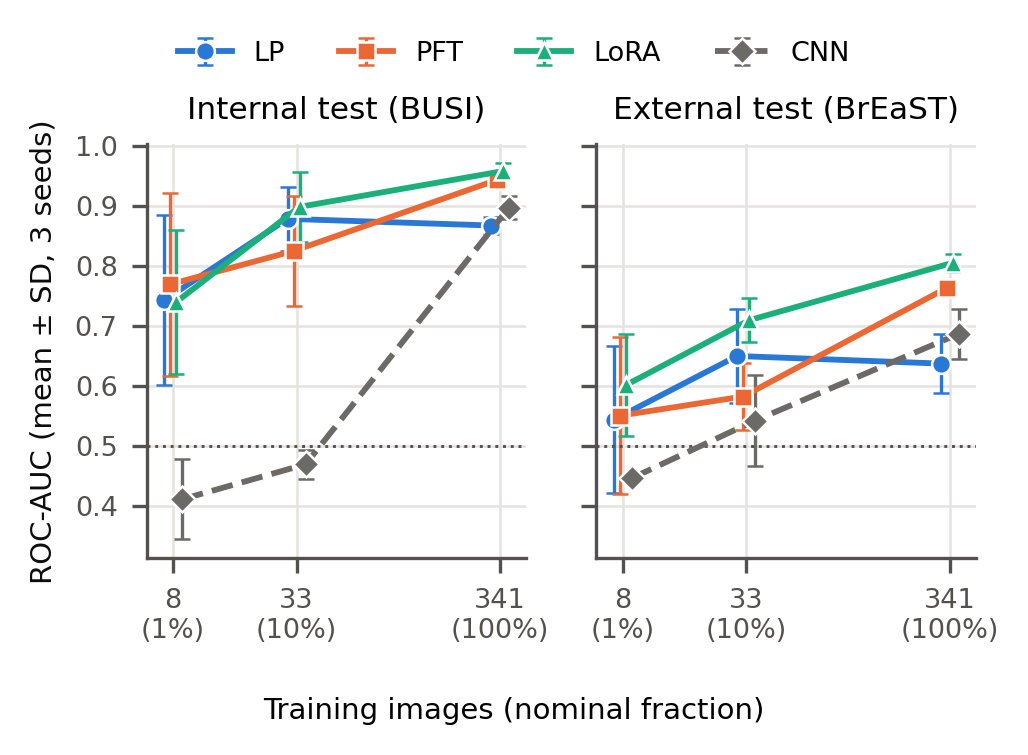
\includegraphics[width=\columnwidth]{fig_learning_curve.png}
\caption{AUC against the number of training images, internal and external test
sets, mean $\pm$ SD over three seeds. The dotted line marks chance.}
\label{fig:learning}
\end{figure}

\begin{table*}[!t]
\caption{Pre-registered contrasts. A difference is detectable only if the
absolute mean difference exceeds the larger per-seed SD \emph{and} the 95\%
interval excludes zero in the same direction. ``gap'' contrasts compare
$\mathrm{AUC}_{\mathrm{in}} - \mathrm{AUC}_{\mathrm{out}}$ between methods.}
\label{tab:contrasts}
\centering
%% Generated by scripts/make_latex.py from tables/. Do not edit.
\scriptsize
\begin{tabular}{llccrrcc}
\toprule
 & Contrast & Labels & Cohort & $\Delta$ mean & Larger SD & 95\% CI of $\Delta$ & Detect. \\
\midrule
H1 & LP $-$ LoRA & 1\% & internal & +0.003 & 0.142 & {[}$-$0.051, +0.056{]} & no \\
H1 & LP $-$ LoRA & 100\% & internal & $-$0.091 & 0.015 & {[}$-$0.156, $-$0.039{]} & yes \\
H2 & LP $-$ PFT & 100\% & internal & $-$0.076 & 0.015 & {[}$-$0.143, $-$0.022{]} & yes \\
H2 & LP $-$ PFT & 100\% & external & $-$0.126 & 0.049 & {[}$-$0.189, $-$0.066{]} & yes \\
H2 & LP $-$ LoRA & 100\% & external & $-$0.168 & 0.049 & {[}$-$0.231, $-$0.110{]} & yes \\
H2 & PFT $-$ LoRA & 10\% & external & $-$0.127 & 0.055 & {[}$-$0.195, $-$0.063{]} & yes \\
H2 & PFT $-$ LoRA & 100\% & external & $-$0.042 & 0.016 & {[}$-$0.077, $-$0.012{]} & yes \\
H2 & LP $-$ PFT & 100\% & gap & +0.050 & 0.059 & {[}$-$0.037, +0.133{]} & no \\
H2 & LP $-$ LoRA & 100\% & gap & +0.077 & 0.059 & {[}$-$0.007, +0.161{]} & no \\
H2 & PFT $-$ LoRA & 100\% & gap & +0.027 & 0.025 & {[}$-$0.017, +0.071{]} & no \\
H3 & LP $-$ CNN & 1\% & internal & +0.332 & 0.142 & {[}+0.196, +0.460{]} & yes \\
H3 & PFT $-$ CNN & 1\% & internal & +0.359 & 0.153 & {[}+0.225, +0.484{]} & yes \\
H3 & LoRA $-$ CNN & 1\% & internal & +0.329 & 0.120 & {[}+0.186, +0.458{]} & yes \\
H3 & LP $-$ CNN & 10\% & internal & +0.410 & 0.053 & {[}+0.276, +0.535{]} & yes \\
H3 & PFT $-$ CNN & 10\% & internal & +0.356 & 0.092 & {[}+0.237, +0.472{]} & yes \\
H3 & LoRA $-$ CNN & 10\% & internal & +0.429 & 0.058 & {[}+0.309, +0.547{]} & yes \\
H3 & LP $-$ CNN & 1\% & external & +0.097 & 0.122 & {[}+0.020, +0.176{]} & no \\
H3 & PFT $-$ CNN & 1\% & external & +0.104 & 0.131 & {[}+0.030, +0.174{]} & no \\
H3 & LoRA $-$ CNN & 1\% & external & +0.155 & 0.085 & {[}+0.085, +0.223{]} & yes \\
H3 & LP $-$ CNN & 10\% & external & +0.108 & 0.079 & {[}+0.033, +0.181{]} & yes \\
H3 & PFT $-$ CNN & 10\% & external & +0.040 & 0.075 & {[}$-$0.058, +0.137{]} & no \\
H3 & LoRA $-$ CNN & 10\% & external & +0.167 & 0.075 & {[}+0.098, +0.234{]} & yes \\
\bottomrule
\end{tabular}

\end{table*}

\subsection{H1: does the ranking depend on the label fraction?}

The two clauses of H1 behave differently (Table~\ref{tab:contrasts}). At 1\%
labels, linear probing and LoRA differ by +0.003 internally, with a 95\%
interval of $[-0.051, +0.056]$ and a per-seed SD of 0.142. The difference is far
smaller than the noise, so it is not detectable. Because we pre-registered no
noninferiority margin, this cannot be read as evidence that the two are
equivalent; the clause is \valVerdictHOneLPNotWorseThanLoRAAtOnePct. At 100\%
labels, LoRA exceeds linear probing internally by 0.091, with an interval of
$[-0.156, -0.039]$ on the LP minus LoRA difference and a much smaller SD, so
that clause is \valVerdictHOneLoRABeatsLPAtHundredPct. Under our compound rule,
H1 as a whole is \textbf{\valVerdictHOne}.

\subsection{H2: is the ranking preserved under center shift?}

At 100\% labels the internal ordering LoRA, PFT, LP does reappear externally:
linear probing is detectably worse than PFT ($-0.126$) and than LoRA ($-0.168$)
on the external cohort, as it is internally. LoRA is detectably better than PFT
externally at 10\% ($-0.127$) and at 100\% ($-0.042$), but the corresponding
internal differences are not detectable, so the two orderings are not the same
statement. At 1\% labels no pair of adaptation strategies is separable in either
cohort. The ranking clause is therefore
\valVerdictHTwoRankingPreservedExternally.

The second clause concerns the gap. None of the three gap contrasts at 100\%
labels is detectable (Table~\ref{tab:contrasts}). The point estimates run
against the clause's worry rather than with it: LP, with \valParamsLP trainable
parameters, has the largest gap (\valMainLPHundredGapMean), while LoRA, with
\valParamsLoRA, has the smallest (\valMainLoRAHundredGapMean). Since no contrast
passes the rule, the clause is
\valVerdictHTwoGapDoesNotGrowWithTrainableParameters and H2 overall is
\textbf{\valVerdictHTwo}.

\subsection{H3: do the foundation-model strategies beat a scratch CNN?}

All six internal contrasts at 1\% and 10\% labels are detectable and in the
predicted direction, with differences between +0.329 and +0.429
(Table~\ref{tab:contrasts}). H3 is \textbf{\valVerdictHThree}. The secondary
external version is weaker: only three of the six contrasts pass the rule, so it
is \valVerdictHThreeExternal.

This verdict needs a caveat that the number alone hides. The margin is produced
mostly by the baseline failing rather than by the foundation model succeeding.
At 1\% and 10\% labels the scratch ResNet-18 scores below chance internally
(\valMainCNNOneAucIn and \valMainCNNTenAucIn), and two of its runs produce
nearly constant probabilities. We checked this for an implementation fault:
reloading each selected checkpoint through the evaluation path reproduces the
logged validation probabilities exactly, and the same code reaches
\valMainCNNHundredAucIn internally with the full training set. Validation AUC at
selection was above chance for every one of those runs, yet the resulting test
AUC is below it, which is what selecting a barely-better-than-random model on a
\valDataBusiVal-image validation set can produce. We read H3 as a statement
about training a network
from scratch on \valDataSubsetOneN to \valDataSubsetTenN images, not as evidence
of strong transfer.

\begin{table*}[!t]
\caption{Cost at the fixed budget, mean $\pm$ SD over three seeds. Charged time
includes the cold feature-extraction cost for LP. ``Cap hit'' counts runs
stopped by the \valProtocolCapSeconds~s deadline.}
\label{tab:cost}
\centering
%% Generated by scripts/make_latex.py from tables/. Do not edit.
\scriptsize
\begin{tabular}{llrrrrccc}
\toprule
Method & Labels & Trainable & Charged (s) & To best (s) & Epochs & Cap hit & Peak RSS (GiB) & Inference (ms/img) \\
\midrule
LP & 1\% & 769 & 19 $\pm$ 1 & 19 $\pm$ 1 & n/a (solver) & 0/3 & 0.59 $\pm$ 0.19 & 183.9 $\pm$ 3.4 \\
LP & 10\% & 769 & 35 $\pm$ 0 & 35 $\pm$ 0 & n/a (solver) & 0/3 & 0.60 $\pm$ 0.20 & 165.9 $\pm$ 1.2 \\
LP & 100\% & 769 & 251 $\pm$ 2 & 251 $\pm$ 2 & n/a (solver) & 0/3 & 0.71 $\pm$ 0.00 & 169.8 $\pm$ 2.3 \\
PFT & 1\% & 3,552,770 & 201 $\pm$ 84 & 101 $\pm$ 77 & 14.7 $\pm$ 5.1 & 0/3 & 0.80 $\pm$ 0.00 & 148.4 $\pm$ 13.0 \\
PFT & 10\% & 3,552,770 & 362 $\pm$ 81 & 227 $\pm$ 91 & 20.7 $\pm$ 4.9 & 0/3 & 1.19 $\pm$ 0.00 & 139.4 $\pm$ 6.0 \\
PFT & 100\% & 3,552,770 & 1228 $\pm$ 201 & 856 $\pm$ 495 & 16.7 $\pm$ 1.5 & 1/3 & 1.20 $\pm$ 0.00 & 134.0 $\pm$ 2.4 \\
LoRA & 1\% & 222,722 & 306 $\pm$ 105 & 198 $\pm$ 97 & 20.7 $\pm$ 5.5 & 0/3 & 1.39 $\pm$ 0.00 & 134.8 $\pm$ 1.1 \\
LoRA & 10\% & 222,722 & 780 $\pm$ 276 & 612 $\pm$ 275 & 35.7 $\pm$ 13.0 & 0/3 & 3.42 $\pm$ 0.01 & 134.8 $\pm$ 1.7 \\
LoRA & 100\% & 222,722 & 1440 $\pm$ 0 & 995 $\pm$ 234 & 12.0 $\pm$ 0.0 & 3/3 & 3.51 $\pm$ 0.01 & 137.1 $\pm$ 1.1 \\
CNN & 1\% & 11,177,538 & 64 $\pm$ 7 & 15 $\pm$ 7 & 10.0 $\pm$ 1.0 & 0/3 & 0.91 $\pm$ 0.00 & 65.1 $\pm$ 2.0 \\
CNN & 10\% & 11,177,538 & 174 $\pm$ 20 & 101 $\pm$ 20 & 18.3 $\pm$ 2.1 & 0/3 & 1.31 $\pm$ 0.02 & 63.1 $\pm$ 0.3 \\
CNN & 100\% & 11,177,538 & 1064 $\pm$ 339 & 705 $\pm$ 383 & 21.7 $\pm$ 6.7 & 1/3 & 1.32 $\pm$ 0.02 & 62.2 $\pm$ 0.6 \\
\bottomrule
\end{tabular}

\end{table*}

\subsection{Cost}

Table~\ref{tab:cost} and Fig.~\ref{fig:cost} show what each method bought with
the budget. Linear probing reached an internal AUC of
\valMainLPHundredAucInMean using \valCostLPHundredTime~s of the
\valProtocolCapSeconds~s available, while LoRA used the entire budget
(\valCostLoRAHundredTime~s) for \valMainLoRAHundredAucInMean and completed only
\valCostLoRAHundredEpochs epochs in that time, against
\valCostPFTHundredEpochs for PFT.

Trainable-parameter counts are a poor proxy for cost here. LoRA trains
\valParamsLoRA parameters against \valParamsPFT for PFT, yet it is the slower
and far heavier of the two: peak resident memory is \valCostLoRAHundredRss~GiB
for LoRA and \valCostPFTHundredRss~GiB for PFT, because gradients still flow
through all 12 blocks. Inference cost inverts the training picture: the three
foundation-model methods all pay the transformer forward pass
(\valCostLPHundredInference~ms per image for LP), while the ResNet-18, which has
the most trainable parameters but is a smaller and cheaper network overall,
predicts in \valCostCNNHundredInference~ms.

\begin{figure}[!t]
\centering
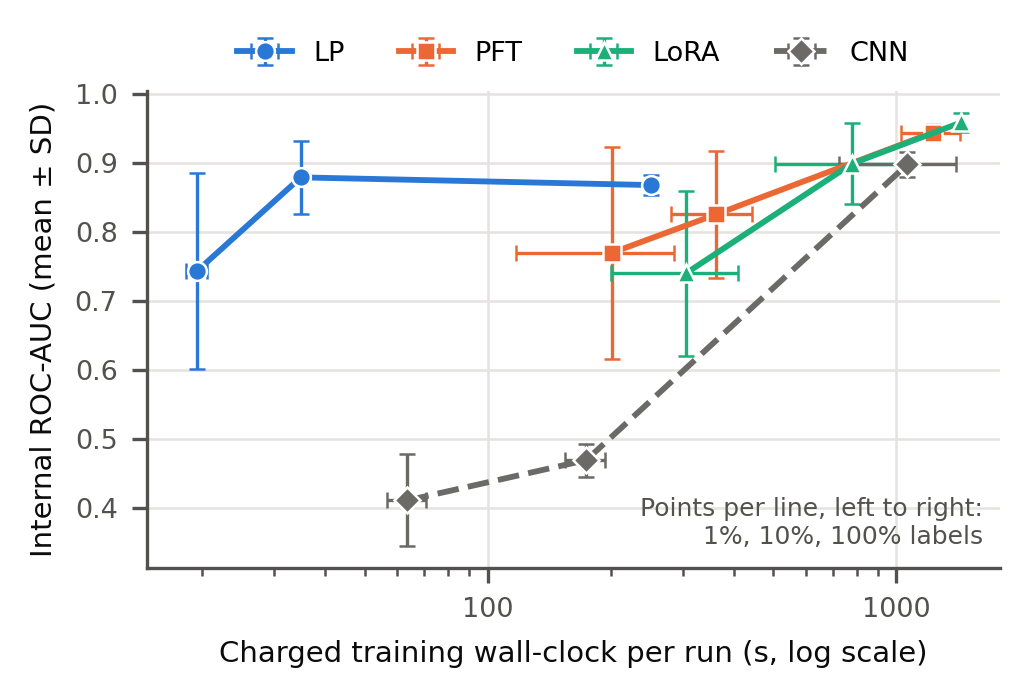
\includegraphics[width=\columnwidth]{fig_cost_performance.png}
\caption{Internal AUC against charged wall-clock time per run, log scale, mean
$\pm$ SD over three seeds.}
\label{fig:cost}
\end{figure}

\subsection{Ablations}

Table~\ref{tab:ablations} and Fig.~\ref{fig:ablations} summarize the ablations.
No ablation changed internal AUC detectably. Four changes were detectable on the
external cohort, and all of them are degradations of LoRA: restricting the
adapters to the last two blocks costs $-0.188$ at 10\% labels and $-0.042$ at
100\%, and changing the rank costs $-0.197$ at rank 4 and $-0.204$ at rank 16.
Removing augmentation ($-0.080$) and deepening PFT to four blocks ($+0.025$)
were not detectable.

Two qualifications limit how far these comparisons can be pushed, and both were
declared before the runs. The hyperparameters were tuned for the main
configuration and reused without retuning, so every ablation is compared against
a configuration that had a tuning advantage. The rank ablation holds $\alpha$
fixed at 16 while varying $r$, so it changes the adapter scaling $\alpha / r$
together with the rank and cannot isolate the two.

\begin{table*}[!t]
\caption{Ablations at the same budget, mean $\pm$ SD over three seeds. Each
variant is contrasted with its own main counterpart on the external cohort under
the pre-registered rule.}
\label{tab:ablations}
\centering
%% Generated by scripts/make_latex.py from tables/. Do not edit.
\scriptsize
\begin{tabular}{llrcclcc}
\toprule
Variant & Labels & Trainable & AUC$_\mathrm{in}$ & AUC$_\mathrm{out}$ & vs. & $\Delta$ AUC$_\mathrm{out}$ [95\% CI] & Detect. \\
\midrule
LoRA, last 2 blocks & 1\% & 38,402 & 0.752 $\pm$ 0.106 & 0.530 $\pm$ 0.042 & LoRA & $-$0.071 {[}$-$0.115, $-$0.028{]} & no \\
LoRA, last 2 blocks & 10\% & 38,402 & 0.846 $\pm$ 0.078 & 0.521 $\pm$ 0.058 & LoRA & $-$0.188 {[}$-$0.248, $-$0.129{]} & yes \\
LoRA, last 2 blocks & 100\% & 38,402 & 0.942 $\pm$ 0.008 & 0.763 $\pm$ 0.016 & LoRA & $-$0.042 {[}$-$0.079, $-$0.007{]} & yes \\
LoRA, rank 4 & 10\% & 112,130 & 0.818 $\pm$ 0.153 & 0.512 $\pm$ 0.055 & LoRA & $-$0.197 {[}$-$0.260, $-$0.131{]} & yes \\
LoRA, rank 16 & 10\% & 443,906 & 0.801 $\pm$ 0.127 & 0.506 $\pm$ 0.114 & LoRA & $-$0.204 {[}$-$0.257, $-$0.153{]} & yes \\
PFT, last 4 blocks & 10\% & 7,103,234 & 0.747 $\pm$ 0.051 & 0.607 $\pm$ 0.048 & PFT & +0.025 {[}$-$0.028, +0.078{]} & no \\
LoRA, no augmentation & 10\% & 222,722 & 0.845 $\pm$ 0.069 & 0.629 $\pm$ 0.121 & LoRA & $-$0.080 {[}$-$0.119, $-$0.045{]} & no \\
\bottomrule
\end{tabular}

\end{table*}

\begin{figure}[!t]
\centering
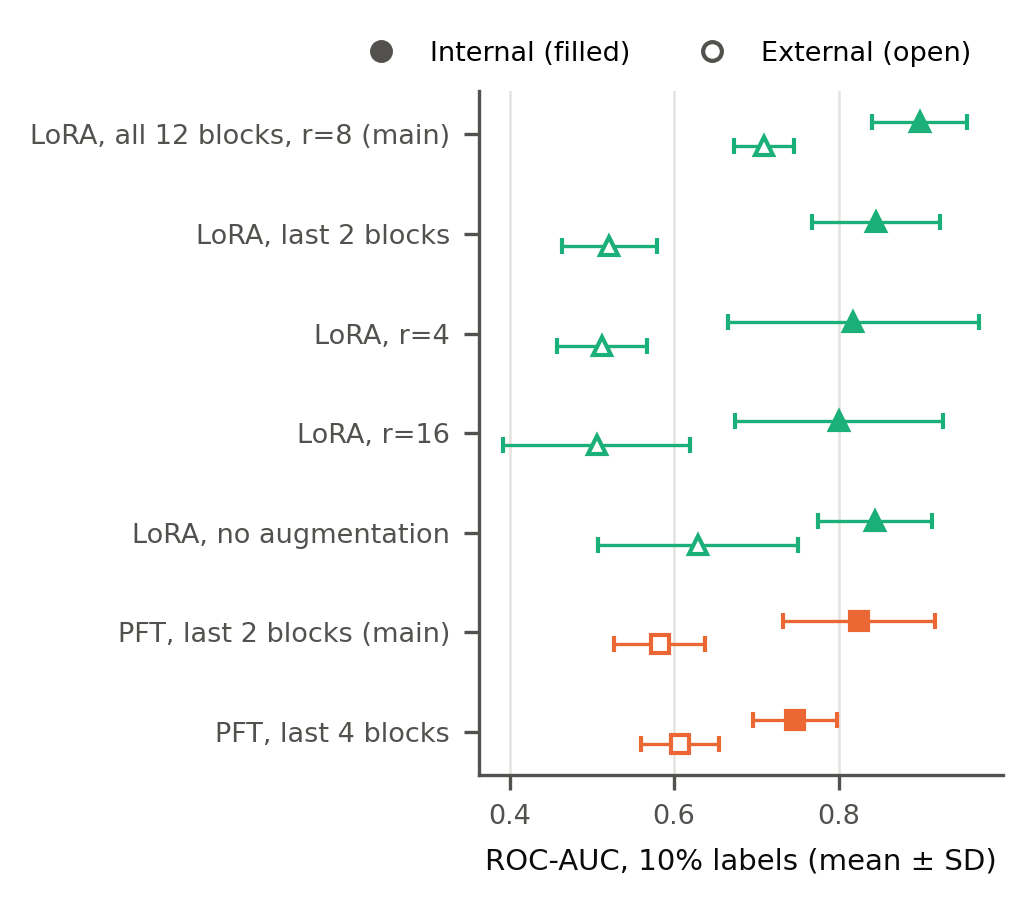
\includegraphics[width=\columnwidth]{fig_ablations.png}
\caption{Ablations at 10\% labels. Filled markers are internal AUC, open markers
external, mean $\pm$ SD over three seeds.}
\label{fig:ablations}
\end{figure}

\subsection{External error typology}

At full labels, \valDataBreastTotal external images divide into 75 that no
method misclassifies in a majority of seeds and 14 that all four get wrong
(Fig.~\ref{fig:overlap}). Method-specific errors are substantial: 27 images are
wrong only for LP and 31 only for the CNN, while 17 are wrong for PFT and LoRA
together, which is consistent with those two sharing an adapted representation.

Stratifying by BI-RADS exposes a difference in \emph{kind}, not only in rate
(Table~\ref{tab:strata}). On BI-RADS 5 lesions, which are almost all malignant,
LP and the CNN are wrong on 0.48 of images while PFT and LoRA are wrong on 0.18
and 0.17. The ordering reverses on clearly benign findings: on BI-RADS 2 the CNN
errs on 0.16 against 0.37 to 0.39 for the three foundation-model methods. The
per-diagnosis table in the released results shows the same split, with LP and
the CNN wrong on 0.51 of invasive carcinomas of no special type against 0.19 and
0.18 for PFT and LoRA, and PFT and LoRA wrong on 0.59 and 0.62 of benign mammary
dysplasia cases against 0.15 for the CNN. Adaptation therefore does not simply
reduce error; at a threshold fixed on internal validation it trades missed
malignancies for false alarms on benign tissue.

We also inspected attention rollout maps for ten deterministically chosen
failures. The maps of the three foundation-model methods are almost identical to
one another, which is expected since all three start from the same pretrained
encoder and change at most a small fraction of its weights, and they are
dominated by a few background tokens. They
therefore carry no information about what adaptation changed, and we draw no
conclusion from them.

\begin{figure}[!t]
\centering
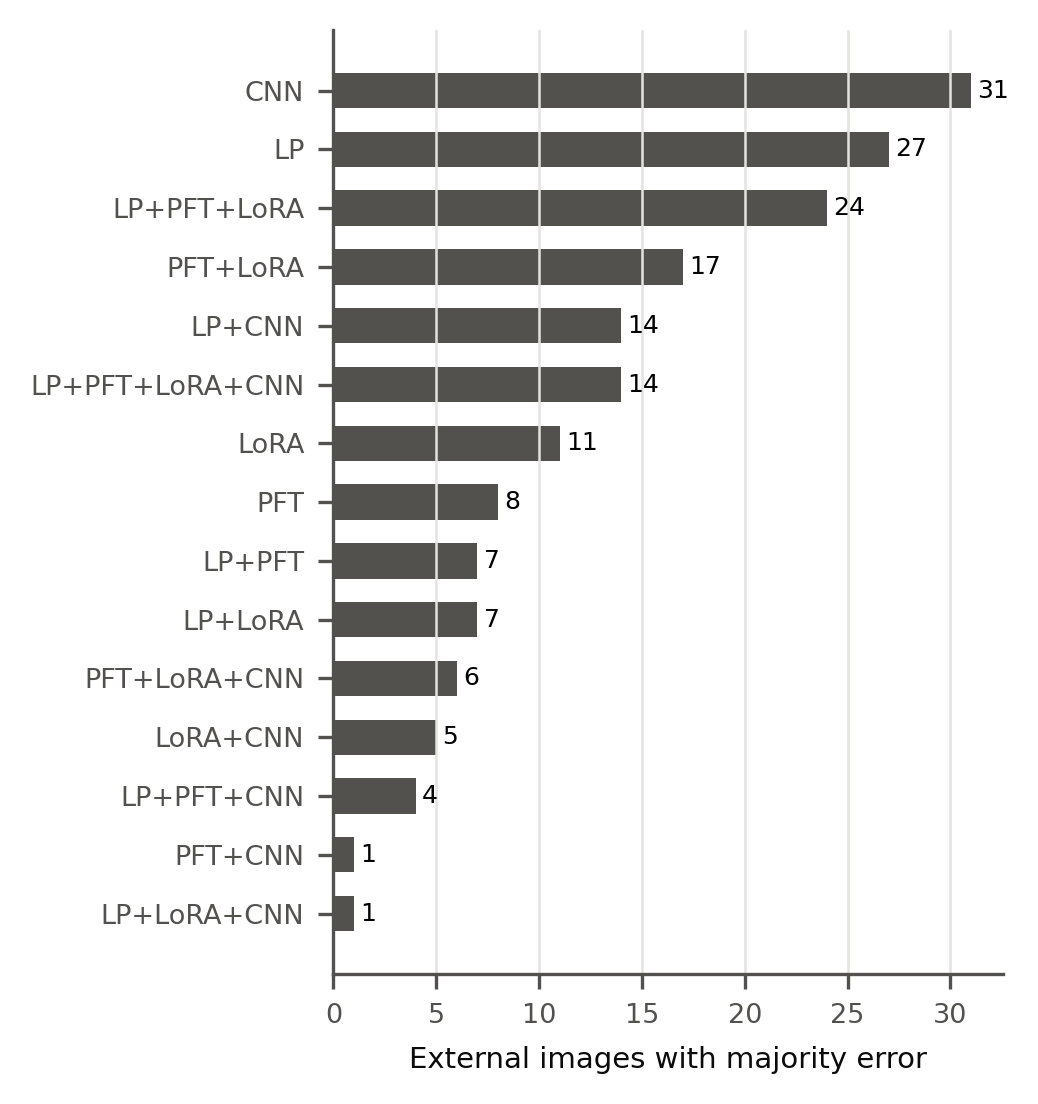
\includegraphics[width=\columnwidth]{fig_error_overlap.png}
\caption{External images at 100\% labels grouped by which methods misclassify
them in a majority of seeds.}
\label{fig:overlap}
\end{figure}

\begin{table}[!t]
\caption{External error rate at 100\% labels by BI-RADS category and
verification route, mean $\pm$ SD over three seeds. ``Malig.'' is the number of
malignant cases in the stratum.}
\label{tab:strata}
\centering
%% Generated by scripts/make_latex.py from tables/. Do not edit.
\footnotesize
\begin{tabular}{lrrcccc}
\toprule
External stratum & $n$ & Malig. & LP & PFT & LoRA & CNN \\
\midrule
BI-RADS 2 & 30 & 0 & 0.37 $\pm$ 0.06 & 0.37 $\pm$ 0.07 & 0.39 $\pm$ 0.16 & 0.16 $\pm$ 0.10 \\
BI-RADS 3 & 37 & 0 & 0.26 $\pm$ 0.06 & 0.17 $\pm$ 0.04 & 0.33 $\pm$ 0.23 & 0.23 $\pm$ 0.18 \\
BI-RADS 4a & 44 & 1 & 0.26 $\pm$ 0.11 & 0.37 $\pm$ 0.06 & 0.39 $\pm$ 0.20 & 0.20 $\pm$ 0.14 \\
BI-RADS 4b & 46 & 16 & 0.35 $\pm$ 0.09 & 0.51 $\pm$ 0.05 & 0.42 $\pm$ 0.11 & 0.35 $\pm$ 0.06 \\
BI-RADS 4c & 49 & 41 & 0.59 $\pm$ 0.02 & 0.33 $\pm$ 0.04 & 0.32 $\pm$ 0.11 & 0.53 $\pm$ 0.23 \\
BI-RADS 5 & 46 & 40 & 0.48 $\pm$ 0.02 & 0.18 $\pm$ 0.03 & 0.17 $\pm$ 0.06 & 0.48 $\pm$ 0.22 \\
Confirmed by biopsy & 197 & 98 & 0.43 $\pm$ 0.05 & 0.34 $\pm$ 0.02 & 0.34 $\pm$ 0.05 & 0.38 $\pm$ 0.05 \\
Confirmed by follow-up care & 55 & 0 & 0.26 $\pm$ 0.04 & 0.26 $\pm$ 0.05 & 0.33 $\pm$ 0.18 & 0.19 $\pm$ 0.12 \\
\bottomrule
\end{tabular}

\end{table}

\subsection{Calibration}

Calibration is worse than discrimination throughout, and it degrades under the
center shift for every method (Table~\ref{tab:main}, Fig.~\ref{fig:reliability}).
At 100\% labels the best-calibrated internal model is PFT
(\valMainPFTHundredEceIn), but the lowest external ECE belongs to the scratch
CNN (\valMainCNNHundredEceOut), ahead of LoRA (\valMainLoRAHundredEceOut) and
far ahead of LP (\valMainLPHundredEceOut); every method's external ECE is worse
than its internal one. Ranking quality and calibration therefore do not order
the methods the same way. At 1\% labels all four methods are badly calibrated in
both cohorts (Table~\ref{tab:main}). Since
the decision threshold is chosen on internal validation and reused unchanged,
these numbers set a practical limit: a model may rank external cases acceptably
and still place its operating point badly.

\begin{figure*}[!t]
\centering
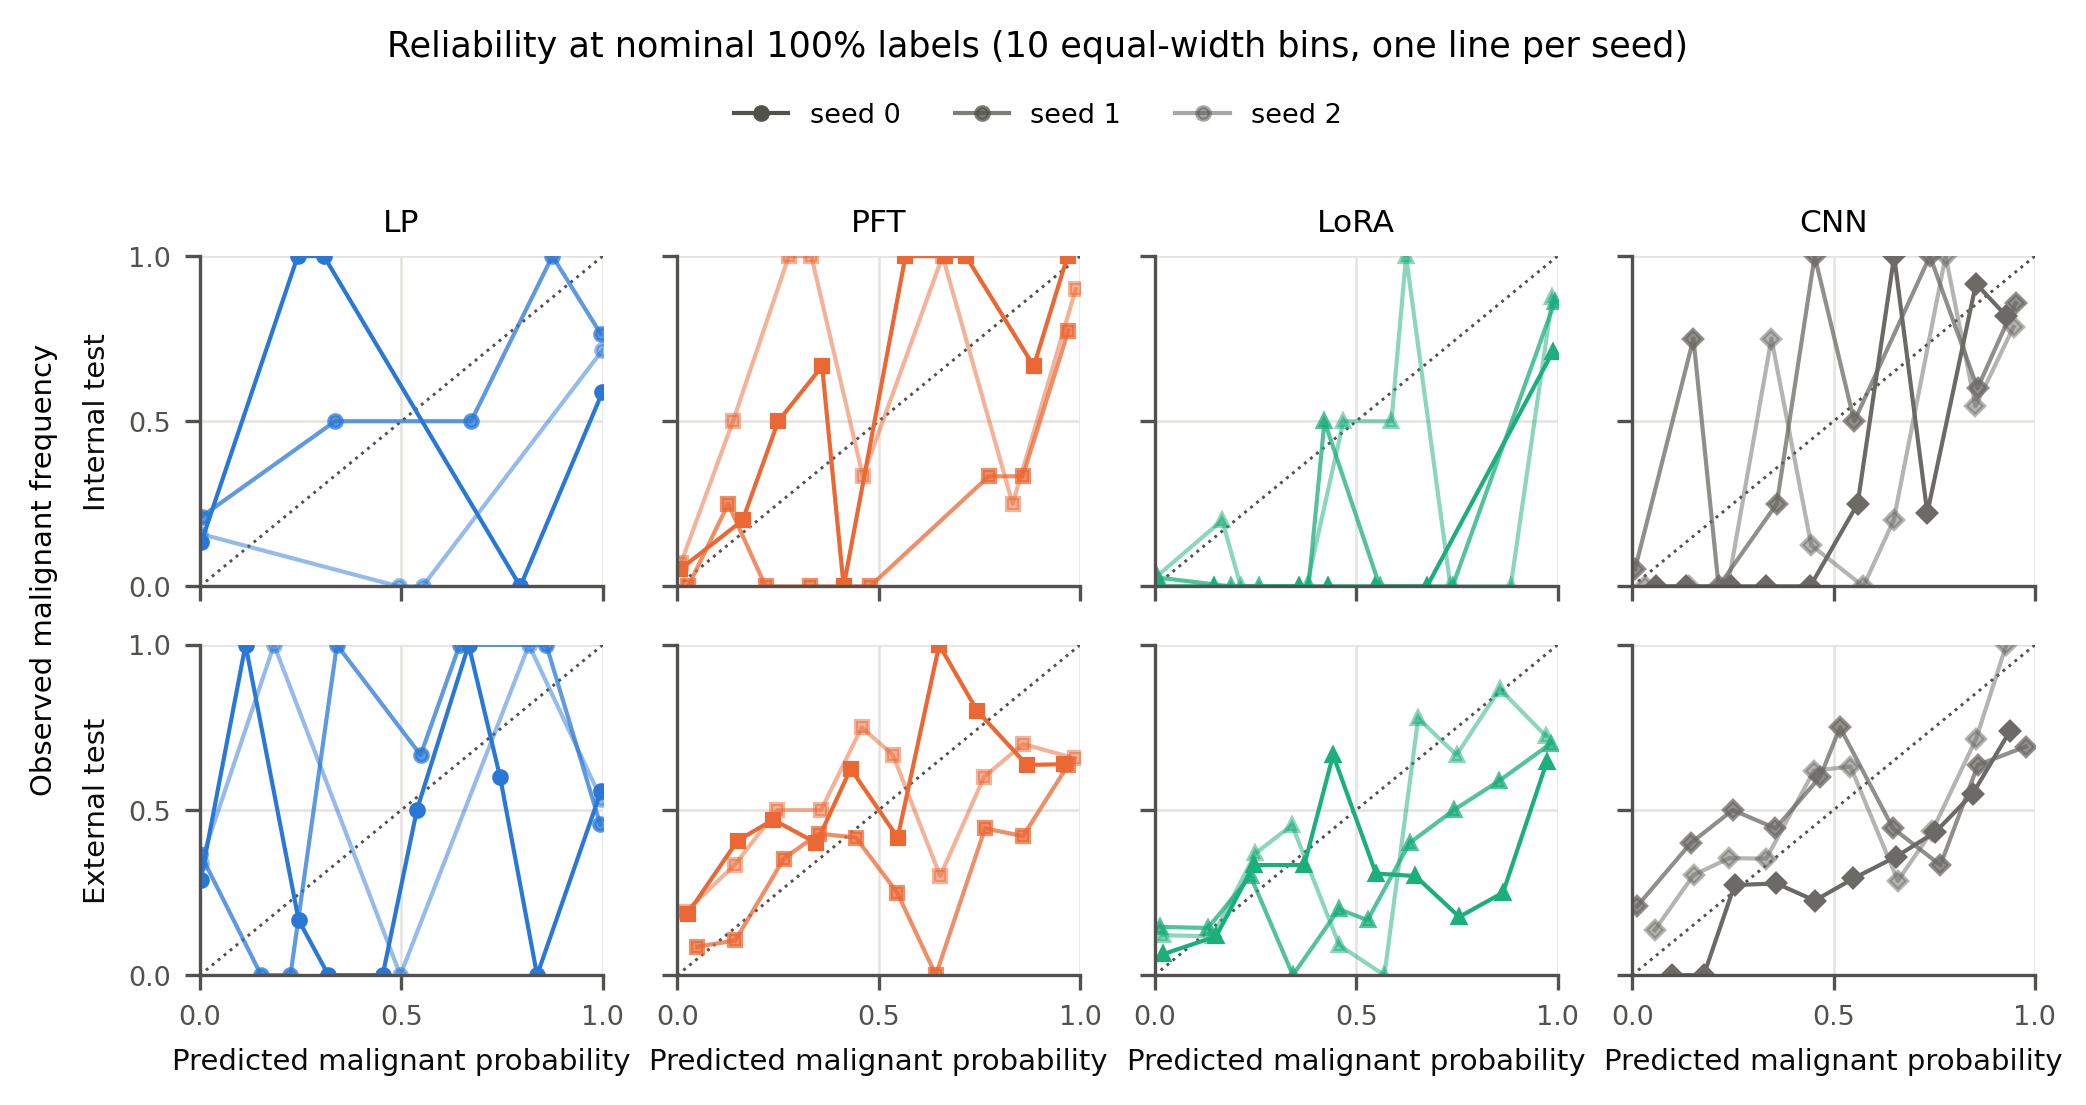
\includegraphics[width=\textwidth]{fig_reliability.png}
\caption{Reliability at 100\% labels, ten equal-width probability bins, one line
per seed. The diagonal is perfect calibration.}
\label{fig:reliability}
\end{figure*}

\subsection{Hypothesis summary}

Table~\ref{tab:hypotheses} collects the verdicts. One of three hypotheses is
supported, none is rejected, and the rest are inconclusive, which under our rule
means the measurement was too noisy to decide rather than that the effects are
absent.

\begin{table}[!t]
\caption{Pre-registered hypotheses and verdicts under the frozen decision rule.
H3$^{*}$ is the secondary external version of H3.}
\label{tab:hypotheses}
\centering
%% Generated by scripts/make_latex.py from tables/. Do not edit.
\footnotesize
\begin{tabular}{lll}
\toprule
 & Clause & Verdict \\
\midrule
H1 & LP not worse than LoRA at 1\% (internal) & \emph{inconclusive} \\
H1 & LoRA beats LP at 100\% (internal) & \emph{supported} \\
\textbf{H1} & \textbf{compound} & \textbf{inconclusive} \\
H2 & Internal ranking preserved externally & \emph{inconclusive} \\
H2 & Gap does not grow with trainable parameters & \emph{inconclusive} \\
\textbf{H2} & \textbf{compound} & \textbf{inconclusive} \\
\textbf{H3} & \textbf{All three FM strategies beat the scratch CNN at 1\% and 10\% (internal)} & \textbf{supported} \\
H3$^{*}$ & Same six contrasts on the external cohort & \emph{inconclusive} \\
\bottomrule
\end{tabular}

\end{table}

\section{Discussion}
\label{sec:discussion}

\textbf{How much adaptation helps depends on having labels at all.} The headline
of our grid is not that one strategy wins but that the question only becomes
answerable once there are enough labels. With the full training set the
measurement is clean: changing the representation, by LoRA or by partial
fine-tuning, is detectably better than a frozen encoder, both internally and on
another center, and linear probing has already stopped improving by 10\% labels.
With \valDataSubsetOneN training images, the seed-to-seed SD is larger than any
difference between strategies, and nothing is separable. For a team with a
handful of labeled scans, our data give no reason to prefer an expensive
adaptation method to a linear probe, and no reason to believe the two are
equivalent either. That is an honest answer to a practical question, but it is a
negative one, and it is a property of this sample size as much as of the methods.

\textbf{The budget binds exactly where the result is most interesting.} All
three LoRA runs at full labels were stopped by the deadline after
\valCostLoRAHundredEpochs epochs. Its reported \valMainLoRAHundredAucInMean is
therefore a lower bound on what LoRA would reach with more time. This cuts two
ways. It strengthens the LoRA-over-LP conclusion, since LoRA wins despite being
truncated. It weakens any claim about LoRA against PFT at full labels, because
PFT stopped early on two of three seeds and was not competing under the same
effective constraint. A budget-matched comparison is not the same as a
convergence-matched one, and at 100\% labels ours is the former.

\textbf{Center shift costs more than the choice of method.} The gap between
cohorts at full labels (\valMainLoRAHundredGapMean to \valMainLPHundredGapMean)
is larger than most of the differences we were testing between methods. No
method's gap is detectably smaller than another's, so we cannot recommend one
adaptation strategy as more robust. We can say that the point estimates do not
support the expectation, from work on feature distortion
\cite{kumar2022distortion}, that adapting more parameters costs more
out-of-distribution accuracy: here the frozen-feature method has the largest gap
and the best external AUC belongs to the method that changes the representation
most widely. Our setting differs from that literature in two ways that could
explain this, namely a very small adapted capacity relative to full fine-tuning,
and a shift that mixes scanner, population and verification rather than a
synthetic corruption.

\textbf{Comparison with PEFT label-efficiency reports.} Studies reporting that
PEFT is particularly valuable in low-data regimes
\cite{lian2024less,dutt2024missed} are not contradicted by our result, but we
cannot confirm them at our smallest budget. Their low-label settings are
typically orders of magnitude larger than \valDataSubsetOneN images, and they do
not equalize wall-clock cost. Our measurement adds the observation that under an
equal CPU budget the advantage of LoRA is visible only once the label count is
large enough for the seed noise to shrink.

\textbf{What the error typology suggests.} The BI-RADS strata show that
adaptation changes which cases fail, not just how many. LP and the scratch CNN
miss malignant, high-BI-RADS lesions; the adapted models catch those and instead
over-call benign mammary dysplasia. In a screening context those two
error profiles have very different consequences, and a single AUC hides the
difference. We report the strata descriptively: they were defined before the
results, but they involve many small groups without multiplicity control, so
they are a hypothesis-generating observation rather than a tested claim.

\subsection{Limitations and threats to validity}

The external set is small (\valDataBreastTotal cases) and the internal test set
smaller still (\valDataBusiTest images), so intervals are wide and small
differences are undetectable by design. The split is image-level: BUSI has no
patient identifiers, so related frames of one patient may still fall in
different splits despite deduplication, which would make internal estimates
optimistic. The center comparison is confounded by scanner, population and
reference standard. The nominal 1\% fraction is really
\valDataSubsetOneActualPct\% of the training data because of the four-per-class
floor, and validation always uses the full validation split, so the low-label
settings consume more labels than their name suggests. We use a single
general-purpose backbone and a binary task without normal images. BUSI images
can carry calipers and text overlays, a known shortcut risk.

The budget is a wall-clock cap on one shared laptop. Concurrent machine load
changed epoch durations: the capped PFT run at 100\% labels had a visibly longer
median epoch than the other two seeds of the same cell at comparable recorded
CPU load, and the available power log cannot detect thermal throttling.
A capped run's epoch count therefore depends on machine state. Training itself
was deterministic: a restarted tuning run reproduced its validation AUCs exactly
for every shared epoch, and an independent retraining of one cell, including
cold feature extraction, reproduced its test AUCs to the logged digits. A CPU
ranking need not transfer to GPU practice, where LoRA's backward cost is
relatively cheaper.

Two departures from ``each test set is read once'' should be stated plainly.
Both happened after all final runs were complete and neither influenced any
selection: one cell was retrained and re-evaluated twice in scratch directories
as a reproducibility check, and the saliency inspection ran forward and gradient
passes over ten external images. Finally, hypothesis verdicts are exploratory
and carry no multiplicity control, and the ablations are compared against a
configuration that was tuned while they were not.

\section{Conclusion}
\label{sec:conclusion}

Under an equal CPU budget of \valProtocolCapMinutes minutes per run, the ranking
of adaptation strategies for a self-supervised vision transformer does depend on
the label fraction, but only at the top of the range. With the full training set
of \valDataBusiTrain images, low-rank adaptation and partial fine-tuning are
detectably better than a linear probe on frozen features, internally and on an
unseen center, and LoRA reaches \valMainLoRAHundredAucIn internally and
\valMainLoRAHundredAucOut externally while using the entire budget. With
\valDataSubsetOneN labeled images no pair of strategies can be told apart, and
our pre-registered rule returns inconclusive rather than equivalence. The
ranking is only partly preserved under the center shift: at full labels every
method loses between \valMainLoRAHundredGapMean and \valMainLPHundredGapMean AUC
on the external cohort, and no method's loss is detectably smaller than
another's. The
one clearly supported hypothesis, that frozen or lightly adapted foundation
features beat a scratch ResNet-18 at low label counts, holds because the
baseline does not learn from so few images.

For practice on commodity hardware our measurement suggests a simple division: a
linear probe is the rational default while labels are scarce or compute is the
binding constraint, and low-rank adaptation is worth its cost only once the
training set is large enough for its advantage to exceed seed noise. For
research, the gap between cohorts remains the dominant term, and closing it is a
more valuable target than further separating these adaptation strategies.

\section*{Use of AI Assistants}

The authors used AI coding assistants, OpenAI Codex and Anthropic Claude Code,
to implement the data pipeline, training and evaluation code, statistical
analysis, figure generation and document build, and to draft and revise text.
Every reference was opened and checked against its source, and every number
reported here is produced by code from logged result files rather than typed by
hand. The authors reviewed the protocol, code and manuscript and remain
responsible for the work.

\section*{Data, Code and License Availability}

Code, the frozen protocol, configurations, logs and result records are provided
as \texttt{SDIA2026\_SAN-1\_GROUP\_13\_code.zip}. Images and model weights are
not redistributed. The preparation scripts fetch BUSI
\cite{aldhabyani2020busi} from a public mirror that states CC0; the original
publication is CC BY 4.0 and we retain its attribution, since a mirror's
metadata cannot alter the original terms. BrEaST-Lesions\_USG
\cite{pawlowska2024breast,pawlowska2024tciadata} is distributed by The Cancer
Imaging Archive under CC BY 4.0, which requires citing both the dataset
(DOI 10.7937/9WKK-Q141) and its descriptor. DINOv2 weights are Apache-2.0
\cite{oquab2024dinov2}. The main libraries are PyTorch, torchvision,
scikit-learn, NumPy, SciPy and pandas (BSD-3-Clause), Transformers and PEFT
(Apache-2.0), Pillow (MIT-CMU), ImageHash (BSD-2-Clause) and Matplotlib (a
PSF-based license); exact versions and license evidence with checksums are in
the released repository.

\bibliographystyle{IEEEtran}
\bibliography{refs}

\end{document}
